%
% chapter.tex -- Gruppen
%
% (c) 2021 Prof Dr Andreas Müller, Hochschule Rapperswil
%
% !TeX spellcheck = de_CH
\chapter{Gruppen
\label{buch:chapter:gruppen}}
\kopflinks{Gruppen}
Die Analyse einer Funktion mit Hilfe einer orthonormierten
Funktionenfamilie trägt der Struktur des Vektorraumes Rechnung.
Falls der Definitionsbereich der Funktionen zusätzliche Symmetrien
hat, lohnt es sich, für die Analyse Funktionen zu verwenden, die
diese Symmetrie zu berücksichtigen.
Zum Beispiel ist der Definitionsbereich $\mathbb{R}$ translationsinvariant,
daher sind Funktionen, die Eigenfunktionen des Translationsoperators
sind, besonders gut geeignet. 
Durch Grenzübergang werden daraus Eigenfunktionen des Ableitungsoperators,
als Funktionen $y(x)$, die die Differentialgleichung $y'(x)=\lambda y(x)$
erfüllen.
Nur die Exponentialfunktionen $y(x)=Ce^{\lambda x}$ sind Lösungen und nur
Exponentialfunktionen der Form $y(x)=e^{ikx}$ mit $k\in\mathbb{R}$
sind beschränkt.
Dies sind genau die Funktionen, die für die komplexe Fourierreihe
verwendet werden.

Die algebraische Struktur einer Gruppe
(Abschnitt~\ref{buch:gruppen:section:gruppe})
fängt die Eigenschaft der Translationsinvarianz ein und ermöglicht
damit die Verallgemeinerung auf weitere Definitionsbereiche.
Zusätzlich wird eine weitere Operation möglich.
Die in Abschnitt~\ref{buch:gruppen:section:faltung} eingeführte
Faltung stattet den Vektorraum der Funktionen auf einer Gruppe
mit einer Multiplikation aus.
Dazu ist ein translationsinvariantes Integral nötig, doch das
Haar-Maß (Abschnitt~\ref{buch:gruppen:section:haar}) zeigt,
dass es ein solches immer gibt.
Die Analyse mit Funktionen, die der Gruppenstruktur Rechnung tragen,
heisst die Gelfand-Transformation
(Abschnitt~\ref{buch:gruppen:section:gelfand})
und hat als natürliche und vielleicht
etwas überraschende Konsequenz die Gültigkeit eines allgemeinen
Faltungssatzes.

Die Gruppenstruktur hält jedoch noch eine weitere Überraschung bereit.
Die Funktionenfamilien, die zur Gelfand-Transformation führen,
sind Spezialfälle von sogenannten Darstellungen, matrixwertigen
Funktionen auf der Gruppe, die die Gruppenoperation respektieren.
Sie werden in Abschnitt~\ref{buch:gruppen:section:darstellung}
eingeführt.
Abschnitt~\ref{buch:gruppen:section:matrixelemente} zeigt, dass
die Matrixelemente einer Darstellung automatisch orthogonale Funktionen
sind.

Die Analyse von Darstellungen lässt sich sogar noch weiter einfacher.
Jede Darstellung lässt sich als Summe von sogenannten irreduziblen
Darstellungen schreiben, die sich nicht weiter zerlegen lassen.
Der Charakter einer Darstellung ist eine Funktion auf der Gruppe.
Es zeigt sich, dass die Charaktere irreduzibler Darstellung eine 
orthonormierte Familie von Funktionen sind.
Die Zerlegung einer Darstellung in irreduzible Summanden wird
dasselbe wie die Zerlegung des Charakters der Darstellung in die
Charaktere der irreduziblen Darstellungen.
Dies wird in Abschnitt~\ref{buch:gruppen:section:charaktere}
dargestellt.


%
% 1-gruppe.tex -- Konzept einer Gruppe
%
% (c) 2022 Prof Dr Andreas Müller, OST Ostschweizer Fachhochschule
%
\section{Gruppen
\label{buch:gruppen:section:gruppe}}
\kopfrechts{Gruppe}
Die Translationsinvarianz des Definitionsbereiches $\mathbb{R}$
entsteht aus der Tatsache, dass die Addition einer Zahl
nicht aus $\mathbb{R}$ herausführt und sich auch umkehren lässt.
Sie basiert also darauf, dass es in $\mathbb{R}$ eine umkehrbare
Verknüpfung gibt.
Diese Idee wird von der algebraischen Struktur einer Gruppe eingefangen.

%
% Definition
%
\subsection{Definition
\label{buch:gruppen:subsection:definition}}
Der Begriff einer Gruppe soll alle Arten von invertierbaren Rechenoperationen
erfassen, also Addition/Subtraktion, Multiplikation/Division oder
die Matrixmultiplikation mit der inversen Matrix.
Die minimal nötigen Eigenschaften fasst die folgende Definition zusammen.

\begin{definition}
\label{buch:gruppen:definition:gruppe}
Eine {\em Gruppe} $G$ ist eine Menge mit einer Verknüpfung
$\cdot \colon G\times G\to G : (x,y) \mapsto xy $, welche folgende
Eigenschaften hat:
\begin{enumerate}
\item
Die Verknüpfung ist assoziativ, d.~h.~$(xy)z=x(yz)$ für alle
$x,y,z\in G$.
\item
Es gibt ein {\em neutrales Element} $e\in G$, für welches $ex=x$ für alle
$x\in G$ gilt.
\index{neutrales Element}%
\item 
Zu jedem $x\in G$ gibt es ein {\em inverses Element} $x^{-1}\in G$ mit der
Eigenschaft $x^{-1}x=e$.
\index{inverses Element}%
\end{enumerate}
\end{definition}

Man beachte, dass die Defiinition nicht verlangt, dass die Faktoren
vertauscht werden können. 

\begin{beispiel}
Die Menge $\operatorname{GL}_n(\mathbb{R})$ der invertierbaren
$n\times n$-Matrizien mit reellen Einträgen und der Matrixmultiplikation
heisst die {\em allgemeine lineare Gruppe}.
\index{allgemeine lineare Gruppe}%
\index{Gruppe!allgemeine lineare}%
Das neutrale Element von $\operatorname{GL}_n(\mathbb{R})$ ist die
Einheitsmatrix, das inverse Element einer Matrix
$A\in \operatorname{GL}_n(\mathbb{R})$
ist die inverse Matrix $A^{-1}$.
\end{beispiel}

\begin{definition}
\label{buch:gruppen:definition:abelsch}
Eine Gruppe $G$ heisst {\em abelsch}, wenn 
$xy=yx$ für alle $x,y\in G$ gilt.
\end{definition}

Die Verknüpfung einer abelschen Gruppe ist also {\em kommutativ}.
Abelsche Gruppen werden oft additiv geschrieben, d.~h.~mit einem
Pluszeichen als $x+y$ für $x,y\in G$.
Das neutrale Element heisst dann auch das {\em Nullelement} und wird $0$
geschrieben: $x+0=x$ für alle $x\in G$.
Das inverse Element von $x$ heisst dann auch das
{\em entgegengesetzte Element} und wird $-x$ geschrieben. 
Es gilt $x+(-x)=0$ für alle $x\in G$.

\begin{beispiel}
Die Gruppe $(\mathbb{R},+)$ ist eine abelsche Gruppe.
Die Gruppe der von $0$ verschiedenen Zahlen mit der Multiplikation
$(\mathbb{R}^*,\cdot)$ ist eine abelsche Gruppe.
\end{beispiel}

%
% Endliche Gruppen
%
\subsection{Endliche Gruppen
\label{buch:gruppen:subsection:endliche-gruppen}}

% XXX Die Gruppen \mathbb{Z}/n\mathbb{Z}
% XXX Die Gruppen S_n

%
% Lie-Gruppen
%
\subsection{Lie-Gruppen
\label{buch:gruppen:subsection:lie-gruppen}}
%
% XXX R und R/Z
% XXX SO(2)
% XXX SO(3) und andere Matrizengruppen

%
% Funktionen auf einer Gruppe
%
\subsection{Funktionen auf einer Gruppe
\label{buch:gruppen:subsection:funktionen}}
In diesem Abschnitt ist $G$ eine Gruppe, die wir multiplikativ
schreiben.
Die harmonische Analysis handelt von der Analyse von Funktionen.
Im Falle einer Lie-Gruppe kann man zusätzlich sinnvoll von Ableitungen
der Funktionen sprechen.
Wir definieren daher

\begin{definition}
Die Menge der stetigen reell- und komplexwertigen Funktionen wird mit
$C_{\mathbb{R}}(G)$ bzw.~$C_{\mathbb{C}}(G)$ bezeichnet.
Ist $G$ eine Lie-Gruppe, dann ist
$C_{\mathbb{R}}^\infty(G)$ die Menge der unendlich oft differenzierbaren
reellwertigen Funktionen auf $G$,
$C_{\mathbb{C}}^\infty(G)$ ist die Menge der unendlich oft differenzierbaren
komplexwertigen Funktionen.
\end{definition}

Die Gruppenstruktur ermöglich, lineare Operatoren auf $C_{\mathbb{R}}(G)$
und $C_{\mathbb{C}}(G)$ zu definieren.

\begin{definition}
Für $s\in G$ ist $T_s$ die Abbildung
\[
T_s
\colon
C_{\mathbb{R}}(G) \to C_{\mathbb{R}}(G)
:
f \mapsto T_sf
\quad
\text{mit}
\quad
(T_sf)(x) = f(s^{-1}x).
\]
Sie heisst die {\em Translation} um $s\in G$.
\end{definition}

Die Translation ist natürlich linear, denn
\begin{align*}
(T_s(f+g))(x)
&=
(f+g)(s^{-1}x)
\\
&=
f(s^{-1}x) + g(s^{-1}x)
=
(T_sf)(x) + (T_sg)(x)
&&\Rightarrow&
T_s(f+g)&=T_sf+T_sg
\\
(T_s(\lambda f))(x)
&=
\lambda f(s^{-1}x)
=
\lambda (T_sf)(x)
&&\Rightarrow&
T_s\lambda f
&=
\lambda T_sf
\end{align*}

%
% Eigenvektoren von T_s
%
\subsubsection{Eigenfunktionen des Translationsoperators}
Tatsächlich wurden in früheren Kapiteln Funktionen verwendet, die
bezüglich der Translation besondere Eigenschaften hatten.
Zum Beispiel sind die Funktionen $f(x)=e_k(x)=e^{ikx}$ auf $G=\mathbb{R}$
Eigenfunktionen des Translationsoperators, denn
\[
(T_se_k)(x)
=
e^{ik(x-s)}
=
e^{iks}e^{ikx}
=
e^{-iks} e_k(x).
\]
Insbesondere ist $e_k$ eine Eigenfunktion von $T_s$ mit Eigenwert
$\lambda=e^{-iks}$, also $T_se_k = \lambda e_k$.

%
% Gruppenstruktur der Translationen
%
\subsubsection{Gruppenstruktur der Translationen}
Wir berechnen die Zusammensetzung zweier Translationen ist $T_s$ und $T_t$.
Um $T_sT_t$ zu berechnen, muss zunächst die Funktion $T_tf$ bestimmt werden.
Es ist $(T_tf)(x) = f(t^{-1}x)$.
Die Translation $T_sg$ einer beliebigen Funktion auf dem Element $y\in G$
ist $(T_sg)(y)=g(s^{-1}y)$.
Setzt man $g=T_tf$ ein, ergibt sich
\[
(T_sT_tf)(x)
=
(T_tf)(s^{-1}x)
=
f(t^{-1}s^{-1}x)
=
f((st)^{-1}x)
=
(T_{st}f)(x),
\]
also $T_sT_t=T_{st}$.

%
% Rechtsoperation der Gruppe auf 
%
\subsubsection{Rechtsoperation von $G$ auf $C(G)$}
Die Operation $T_s$ ist genauer die Links-Translation, die Gruppenoperation
wirkt auf das Argument von links.
Für eine abelsche Gruppe spielt die Reihenfolge der Operanden keine
Rolle, für eine nichtabelsche Gruppe ergibt sich jedoch ein Unterschied.

\begin{definition}
Der Operator $R_s\colon C(G)\to C(G)$ der Rechts-Translation ist definiert
durch
\[
R_s
\colon
C_{\mathbb{R}}(G)\to C_{\mathbb{R}}(G)
:
f \mapsto R_sf
\quad\text{mit}\quad
(R_sf)(x) = f(xs).
\]
\end{definition}

Die Zusammensetzung von $R_s$ und $R_t$ kann ganz ähnlich wie für
$T_s$ und $T_t$ berechnet werden.
Zunächst ist $R_sg(y) = g(ys)$.
Wendet man dies auf $g=R_tf$ mit $g(x)=(R_tf)(x)=f(xt)$ an, bekommt man
\[
(R_sR_tf)(x)
=
(R_sg)(x)
=
g(xs)
=
(R_tf)(xs)
=
f(xst)
=
(R_{st}f)(x)
\]
oder kurz $R_sR_t=R_{st}$.







%
% 2-haar.tex -- Haar-Mass
%
% (c) 2022 Prof Dr Andreas Müller, OST Ostschweizer Fachhochschule
%
\section{Haar-Mass
\label{buch:gruppen:section:haar}}
\kopfrechts{Haar-Mass}
Die Integration von Funktionen einer reellen Variablen oder auch
das in Abschnitt
\ref{buch:skalarprodukt:funktionenraeume:subsection:grenzen-riemann}
erwähnte Lebesque-Integral hat die Eigenschaft, dass das
Integral einer Funktion sich nicht ändert, wenn man die Funktion
entlang der reellen Achse verschiebt.
Für eine integrierbare Funktion $f\colon\mathbb{R}\to\mathbb{R}$
gilt
\[
\int_{-\infty}^\infty f(x)\,dx
=
\int_{-\infty}^\infty f(x-s)\,dx
=
\int_{-\infty}^\infty T_sf(x)\,dx,
\]
wobei die $T_s$ die in Definition~\ref{buch:gruppen:gruppe:def:translation}
eingeführt Translationsoperation ist.
Die harmonische Analysis mit den Exponentialfunktion $e^{ikx}$ 
verwendet diese Translationsinvarianz der Integration auf wesentliche Art,
das Skalarprodukt von Funktionen ändert sich ebenfalls nicht, wenn sie
entlang der $t$-Achse verschoben werden.

Wenn die harmonische Analysis auf andere Gruppen als auf die reellen
Zahlen ausgedehnt werden soll, dann wird eine Integration auf diesen
Gruppen benötigt, welche die gleiche Invarianzeigenschaft unter
Translationen hat.

%
% Mittelung auf einer endlichen Gruppe
%
\subsection{Mittelung auf einer endlichen Gruppen
\label{buch:haar:subsection:endlich}}
Für endliche Gruppen ist es nicht schwierig eine invariante
``Integration'' zu konstruieren.
Da die Gruppe nur aus isolierten Punkten besteht, muss jedes Element das 
gleiche Gewicht $1/|G|$ haben.
Die invariante Integration ist also nichts anderes als eine
Mittelwertbildung.

\begin{definition}
\label{buch:gruppen:haar:def:mittelung}
Sei $G$ ein endliche Gruppe und $f$ eine Funktion $f\colon G\to \mathbb{R}$.
Die {\em Mittelungsoperation} über die Gruppe ist die Operation
\[
Mf = \frac{1}{|G|}\sum_{g\in G} f(g).
\]
\index{Mittelungsoperation}
\end{definition}

Die Mittelungsoperation ist natürlich linear, denn
\[
M(\lambda f + \mu g)
=
\frac{1}{|G|}
\sum_{h\in G}
(\lambda f(h)+\mu g(h))
=
\lambda \frac{1}{|G|}\sum_{h\in G}f(h)
+
\mu \frac{1}{|G|}\sum_{h\in G}g(h)
=
\lambda Mf + \mu Mg.
\]
Die Operation ist aber auch translationsinvariant.
Dazu muss
\begin{equation}
MT_sf
=
\frac{1}{|G|}
\sum_{g\in G} f(s^{-1}g)
\label{buch:gruppen:haar:eqn:mitteltranslation}
\end{equation}
mit $Mf$ verglichen werden.
Die Abbildung $g\mapsto s^{-1}g$ ist aber nur eine Permutation der endlich
vielen Elemente der Gruppe $G$.
Die Summe auf der rechten Seite von
\eqref{buch:gruppen:haar:eqn:mitteltranslation}
ist daher nur die Summe über alle Funktionswerte $f(g)$ in einer anderen
Reihenfolge oder
\[
MT_sf
=
\frac{1}{|G|} \sum_{g\in G}f(g)
=Mf.
\]
Damit ist gezeigt, dass die Mittelungsoperation translationsinvariant
ist.

Die Mittelungsoperation von Definition~\ref{buch:gruppen:haar:def:mittelung}
ermöglicht jetzt, das translationsinvariante Skalarprodukt
\[
\langle f,g\rangle_G
=
M(\overline{f}g)
=
\frac{1}{|G|}
\sum_{h\in G}
\overline{f(h)}g(h)
\]
zu definieren.

Im Nachweis, dass die Mittelungsoperation invariant ist bezüglich
der Translation wurde ausschliesslich verwendet, dass die Abbildung
$g\mapsto s^{-1}g$ ein Permutation der Gruppenelemente ist.
Die Rechtstranslation $R_s\colon g\mapsto gs$ ist ebenfalls eine
Permutation, es folgt also, dass die Mittelungsoperation auch
bezüglich der Rechtstranslation invariant ist.

%
% Integration auf Lie-Gruppen
%
\subsection{Integration auf Lie-Gruppen
\label{buch:haar:subsection:lie-gruppen}}
Die Gruppe der reellen Zahlen ist auch ein Lie-Gruppe, da sie eine
eindimensionale Mannigfaltigkeit ist und die Translationsoperation
eine differenzierbare Abbildung ist.
Die Translationsinvarianz bedeutet dann, dass man einen Massstab für
die Längenmessung durch Translation vom Nullpunkt an jeden beliebigen
anderen Punkt von $\mathbb{R}$ transportieren kann.
Der Transport mit $T_s$ ist die Variablentransformation $x\mapsto x-t$,
die $dx$ in $dx$ überführt, das Integral also unverändert lässt.

Diese Idee lässt sich auf beliebige Lie-Gruppen übertragen.
Um ein Integral auf der Lie-Gruppe zu definieren, muss man in jedem
Punkt ein Koordinatensystem haben und ausserdem wissen, wie die
Integration bezüglich dieses Koordinatensystems durchzuführen ist,
man braucht das ``Volumenelement'' ausgedrückt in diesen Koordinaten.

Wir betrachten ein Koordinatensystem mit Koordinaten $x_1,\dots,x_n$
in einer Umgebung $U$ des neutralen Elementes $e$ einer Lie-Gruppe $G$.
Das Integral
\[
\int_{U} f(x_1,\dots,x_n) \,dx_1\,\dots\,dx_n
\]
der Funktion $f$ in der Umgebung $U$ ist aber nicht unbedingt
translationsinvariant.
Für ein Gruppenelement $s$ nahe beim neutralen Element der Gruppe
ist die Translation mit $T_s$ eine Koordinatentransformation
$(x_1,\dots,x_n)\mapsto (x_1',\dots,x_n')$.
Das Integral kann auch in den gestrichenen Koordinaten als
\[
\int_{U} f(x_1,\dots,x_n) \,dx_1\,\dots\,dx_n
=
\int_{U'} f(x_1',\dots,x_n')
\frac{\partial (x_1,\dots,x_n)}{\partial(x_1',\dots,x_n')}
\,dx_1'\,\dots\,dx_n'
\]
berechnet werden.
Die Funktionaldeterminante hängt natürlich von $s$ ab.
Die Integrale unterscheiden sich nur durch eine skalare Gewichtsfunktion.
Durch geeignete Wahl einer Funktion $w(x_1,\dots,x_n)$ kann man 
das Integral
\[
\int_{U} f(x_1,\dots,x_n) w(x_1,\dots,x_n)\,dx_1\dots\,dx_n
\]
mindestens in einer Umgebung des neutralen Elementes
translationsinvariant machen.

Möglicherweise gibt es kein globales Koordinatensystem für die 
die Gruppe $G$, aus diesem Grund wurde ja das Konzept der Karte
und des Atlas eingeführt.
Das Koordinatensystem in einer Umgebung des neutralen Elements und
die zugehörige translationsinvariante Integration kann aber mit
dem Operator $T_s$ in jeden beliebigen anderen Punkt $s$ transportiert
werden.
In einer Umgebung von $s$ gibt es daher ebenfalls eine
translationsinvariante Integration.
Da es nur genau ein einziges Element in $G$ gibt, welches die Translation
von $e$ nach $s$ ausführen kann, ist diese translationsinvariante 
Integration auf der ganzen Gruppe wohldefiniert.

Wir schliessen daher, dass es auf einer Lie-Gruppe ganz analog 
zu den reellen Zahlen eine translationsinvariante Integration
gibt.

\begin{beispiel}
Die Lie-Gruppe $S^1 = \operatorname{SO}(2)$ der Drehungen in der Ebene
kann mit dem Drehwinkel parametrisiert werden:
\[
g(x)
=
\begin{pmatrix*}[r]
\cos x&-\sin x\\
\sin x& \cos x
\end{pmatrix*}
\in
\operatorname{SO}(2)
\]
Die Koordinaten $x$ ist also ein mögliches Koordinatensystem in einer
Umgebung des neutralen Elementes.
Als Koordinatensystem für die ganze Gruppe ist problematisch daran,
dass das gleiche Gruppenelement für viele verschiedene $x$-Werte
erreicht wird, nämlich für alle, die sich um ein ganzzahliges
Vielfaches von $2\pi$ unterscheiden.
Die $x$-Werte im Intervall $[0,2\pi)$ beschreiben also alle Elemente
der Gruppe $\operatorname{SO}(2)$. 

Die Koordinatentransformation, die mit der Translation $T_s$ einhergeht,
ist die Abbildung $x\mapsto x-s$, die die Funktionaldeterminante $1$
hat.
Die Integration
\[
\int_{\operatorname{SO}(2)} f(g) \,dg
=
\int_0^{2\pi} f(g(x))\,dx
\]
ist daher eine translationsinvariante Integration.
Jedes skalare Vielfache davon ist aber ebenfalls eine translationsinvariante
Integration.
Die Integration
\[
f
\mapsto
\frac{1}{2\pi}\int_0^{2\pi} f(g(x))\,dx
\]
hat die nützliche Eigenschaft, dass die konstante Funktion $1$ das
Integral $1$ hat.
\end{beispiel}

%
% Das Haar-Mass
%
\subsection{Das Haar-Mass
\label{buch:haar:subsection:haar}}
Man kann zeigen, dass die Konstruktion, die im vorangegangenen Abschnitt
für Lie-Gruppen mit ihrer differenzierbaren Struktur auch wesentlich
abstrakter für beliebige topologische Gruppen durchgeführt werden kann.
Sie geht auf Alfred Haar zurück.

\begin{satz}[Haar]
\label{buch:gruppen:haar:satz:haar}
Ist $G$ eine lokal kompakte, topologische Gruppe, dann gibt es ein
translationsinvariantes Mass $\mu$ auf $G$, also ein Mass derart,
dass 
\[
\int_G f(g)\,d\mu(g)
=
\int_G T_sf(g)\,d\mu(g)
=
\int_G f(s^{-1}g)\,d\mu(g)
\]
gilt für alle $s\in G$.
Das Mass $\mu$ ist bis auf einen skalaren Faktor eindeutig bestimmt.
\end{satz}

Man beachte die Voraussetzung, dass die Gruppe lokal kompakt sein
muss.
Damit wird erreicht, dass sich die Gruppe lokal ähnlich wie ein
endlichdimensionaler Vektorraum verhält.
Sie sorgt zum Beispiel dafür, dass es immer eine offene Umgebung
$U$ eines Punktes gibt, die endliches Volumen $\mu(U)$ hat.

Das im Satz~\ref{buch:gruppen:haar:satz:haar} definierte Mass
heisst das {\em linksinvariante haarsche Mass}.
\index{haarsches Mass!linksinvariant}%
Die Voraussetzung {\em lokal kompakt} ist eine Endlichkeitsbedingung,
\index{Endlichkeitsbedingung}%
die unendlichdimensionale Gruppen ausschliesst.
Sie verlangt, dass jeder Punkt eine kompakte Umgebung hat, dass also
in der Nähe eines Punktes die Gruppe wie ein endlichdimensioinaler 
Raum aussieht.

Die Konstruktion, die auf Satz~\ref{buch:gruppen:haar:satz:haar}
führt, kann auch für die Rechtstranslation mit $R_s$ durchgeführt
werden.
Es gibt also auf einer topologischen Gruppe auch ein bis auf einen
skalaren Faktor eindeutig bestimmtes rechtsinvariantes haarsches Mass,
der Satz sagt aber nichts darüber aus, ob das linksinvariante und das
rechtsinvariante Mass übereinstimmen.

%
%  Stetige Funktionen mit kompaktem Träger
%
\subsubsection{Stetige Funktionen mit kompaktem Träger}
Da die Gruppe nicht komapkt sein muss ist es durchaus möglich,
dass sogar eine beschränkte stetige Funktion auf $G$ ein divergentes
Integral hat.
Dies kann vermieden werden, wenn man nur Funktionen zulässt, die
nur auf einem kompakten Gebiet von $0$ verschieden sind.

\begin{definition}
Der Vektorraum der Funktionen mit kompaktem Träger wird mit
\[
\mathscr{K}(G)
=
\{ f\in C(G)\mid \text{$\operatorname{supp}f $ ist kompakt}\}
\]
bezeichnet.
\end{definition}

Im Unterraum $\mathscr{K}(G)\subset C(G)$ ist die Integration
immer durchführbar.

%
% Unimodulare Gruppen
%
\subsection{Unimodulare Gruppen
\label{buch:haar:subsection:unimodular}}
Für eine abelsche Gruppe, wie die Gruppe der reellen Zahlen
oder $\mathbb{R}^n$, gibt es keinen Unterschied zwischen Links- und
Rechtstranslation, daher sind auch die links- und rechtsinvarianten
haarschen Masse identisch.
Die Mittelungsoperation einer endlichen Gruppe ist sowohl rechts-
als auch linksinvariant, selbst dann, wenn die Gruppe nicht abelsch
ist.
Für eine nicht kommutative Gruppe wie die Gruppe $\operatorname{SO}(3)$
der Drehungen des Raumes dagegen ist es nicht mehr klar, dass 
die rechts- und linksinvarianten Masse gleich sein müssen.

Sei $G$ eine Gruppe mit dem linksinvarianten Mass $\mu$.
Dann ist $R_s\mu$ ebenfalls ein linksinvariantes Mass definiert
durch das Integral
\[
\int_G f(g) \, dR_r\mu(g)
=
\int_G R_rf(g) \,d\mu(g)
=
\int_G f(gr)\,d\mu(g).
\]
Setzen wir darin $T_sf$ ein, zeigt sich, dass wegen
\[
\int_G T_sf(gr)\,d\mu(g)
=
\int_G f(s^{-1}gr)\,d\mu(g)
=
\int_G f(gr)\,d\mu(g)
\]
$R_r\mu$ ein linksinvariantes Mass ist.
Nach dem Satz~\ref{buch:gruppen:haar:satz:haar} unterscheiden sich
die beiden Masse um einen skalaren Faktor.

\begin{definition}[unimodular]
Es gibt eine Funktion $\delta\colon G\to \mathbb{R}$ derart, dass
\[
R_r \mu = \delta(r) \mu
\]
für $r\in G$
ist.
Die Gruppe $G$ heisst {\em unimodular}, wenn $\delta(r)=1$ ist für
\index{unimodular}
alle $r\in G$.
\end{definition}

Für eine unimodulare Gruppe unterscheiden sich die linksinvarianten
und die rechtsinvarianten Masse also nicht.
Abelsche Gruppen sind unimodular.
Man kann auch zeigen, dass $\delta(r)$ ein Homomorphismus in die
multiplikative Gruppe $\mathbb{R}^*$ ist,
was sich als ziemlich starke Einschränkung herausstellt.
Sie ist verwandt mit der Determinanten auf einer Matrizengruppe.

\begin{satz}
Ist die lokalkompakte topologische Gruppe $G$ sogar kompakt, dann ist
sie unimodular.
\end{satz}

\begin{proof}[Beweis]
Die Funktion $\delta\colon G\to\mathbb{R}$ ist ein stetiger Homomorphismus.
Als stetige Funktion hat sie auf dem kompakten Definitionsbereich $G$
mindestens ein Maximum und ein Minimum.
Wir bezeichen die Stellen des Maximums mit $g$.
Wenn $\delta(g)>1$ wäre, dann wäre auch
\[
\delta(gg)
=
\delta(g)
\delta(g)
>
\delta(g),
\]
der Wert an  der Stelle $gg$ wäre also grösser als das Maximum.
Der Widersprich zeigt, dass das Maximum $\delta(g)=1$ sein muss.
Analog sieht man ein, dass auch das Minimum von $\delta(g)=1$
sein muss, dass also $\delta(g)=1$ ist.
\end{proof}

\begin{beispiel}
Die Gruppe der Streckungen und Verschiebungen 
\[
G
=
\mathbb{R^+}\ltimes \mathbb{R}
\]
besteht aus Paaren $(s,t)$ mit der Verknüpfung
\[
(s_1,t_1)\cdot(s_2,t_2)
=
(s_1s_2,t_1 + s_1t_2).
\]
Die zweite Komponente im Produkt ist offensichtlich nicht symmetrisch
in den beiden Indizes $1$ und $2$, die Gruppe $G$ ist nicht abelsch.
Das inverse Element von $(s,t)$ ist $(s^{-1},-s^{-1}t)$, denn
\begin{align*}
(s,t)\cdot(s^{-1},-s^{-1}t)
&=
(ss^{-1}, t-ss^{-1}t)
=
(1,0)
\\
(s^{-1},-s^{-1}t)\cdot(s,t)
&=
(s^{-1}s,-s^{-1}t+s^{-1}t)
=
(1,0).
\end{align*}
Das linksinvariante haarsche Mass muss von der Form
\[
\int_G f(g) w(g)\,dg
=
\int_0^\infty \int_{-\infty}^\infty
f(\sigma,\tau)
w(\sigma,\tau)
\,d\tau\,d\sigma
\]
sein,
die Gewichtsfunktion $w(\sigma,\tau)$ muss noch bestimmt werden.
Die Linkstranslation mit $(s,t)$ ist 
\begin{align*}
\int_G f(h^{-1}g) w(g)\,dg
&=
\int_0^\infty
\int_{-\infty}^\infty
f((s^{-1},-s^{-1}t)(\sigma,\tau)\,
w(\sigma,\tau)
\,d\tau
\,d\sigma
\\
&=
\int_0^\infty
\int_{-\infty}^\infty
f(s^{-1}\sigma,-s^{-1}t+s^{-1}\tau)\,
w(\sigma,\tau)
\,d\tau
\,d\sigma.
\intertext{Wir schreiben $\sigma'=s^{-1}\sigma$ und
$\tau'=-s^{-1}t+s^{-1}\tau$ oder gleichbedeutend
$\sigma=s\sigma'$ und $\tau=s\tau'+t$ und bekommen
}
&=
\int_{0}^\infty
\int_{-\infty}^\infty
f(\sigma',\tau')\,
w(s\sigma',s\tau'+t)
\,s\,d\tau'
\,s\,d\sigma',
\intertext{
dabei wurde $d\tau = s\,d\tau'$ und $d\sigma=s\,d\sigma'$ verwendet.
Linksinvarianz würde bedeuten, dass dieses Integral für
alle Funktionen $f$ übereinstimmt mit}
&=
\int_{0}^\infty
\int_{-\infty}^\infty
f(\sigma',\tau')\,
w(\sigma',\tau')\, s^2
\,d\tau'
\,d\sigma'.
\end{align*}
Es folgt, dass die Funktion $w$ die Funktionalgleichung
\[
w(s\sigma',s\tau'+t) = w(\sigma',\tau') s^2
\]
für alle $s$ und $t$ erfüllen muss.
Da man $t$ beliebig verändern kann folgt,
dass $w$ nicht vom zweiten Argument abhängt, dass also
$w(\sigma',\tau') = w(\sigma')$.
Aus $\sigma'=1$ folgt dann $w(s)=w(1)s^2$, oder.
$w(s,t)=as^2$.

Für die Rechtsinvarianz suchen wir ganz analog eine Funktion
$\tilde{w}(s,t)$ derart, dass
\begin{align*}
\int_0^\infty
\int_{-\infty}^\infty
f(\sigma,\tau)
\,\tilde{w}(\sigma,\tau)
\,d\sigma\,d\tau
&=
\int_0^\infty
\int_{-\infty}^\infty
f((\sigma,\tau)\cdot(s,t))
\,\tilde{w}(\sigma,\tau)
\,d\sigma\,d\tau
\\
&=
\int_0^\infty
\int_{-\infty}^\infty
f(\sigma s,\tau +\sigma t)
\,\tilde{w}(\sigma,\tau)
\,d\sigma\,d\tau.
\intertext{Wie vorhin verwenden wir die Substitution $\sigma'=s\sigma$ und
$\tau' = \tau+\sigma t$ oder umgekehrt $\sigma=s^{-1}\sigma'$  und
$\tau = \tau' - \sigma t = \tau' - s^{-1}t\sigma'$ und erhalten}
&=
\int_0^\infty
\int_{-\infty}^\infty
f(\sigma',\tau')
\,
\tilde{w}(s^{-1}\sigma', \tau'-\sigma t)
\,d\sigma\,d\tau.
\\
&=
\int_0^\infty
\int_{-\infty}^\infty
f(\sigma',\tau')
\,
\tilde{w}(s^{-1}\sigma', \tau'-\sigma t)
\,s^{-1}\,d\sigma'
\,d\tau'.
\end{align*}
Dies muss für beliebige $(s,t)$ und beliebige Funktionen gelten,
woraus man schliessen kann, dass $\tilde{w}$ die Funktionalgleichung
\[
\tilde{w}(\sigma',\tau')
=
\tilde{w}(s^{-1}\sigma', \tau'-s^{-1}\sigma't)\,s^{-1}
\]
erfüllt.
Wieder folgt, dass $\tilde{w}$ nicht vom zweiten Argument abhängt, und
die Abhängigkeit vom ersten Argument ist $\tilde{w}(s,t)=s$.

Da die beiden Funktionen $w(s,t)$ und $\tilde{w}(s,t)$ verschieden sind,
sind das rechtsinvariante und das linksinvariante Haar-Mass verschieden
und die Gruppe $G$ ist nicht unimodular.
\end{beispiel}

Die Tatsache dass $\mathbb{R}^+\ltimes\mathbb{R}$ nicht kompakt
und nicht abelsch ist, ist nicht ein ausreichender Grund zu
schliessen, dass $G$ nicht unimodular sein könne.
Wir werden später die Gruppe der Drehungen und Verschiebungen
$\operatorname{SO}(2)\ltimes \mathbb{R}^2$ kennenlernen,
die ebenfalls nicht abelsch und nicht kompakt aber trotzdem
unimodular ist.

%
% 3-faltung.tex
%
% (c) 2022 Prof Dr Andreas Müller, OST Ostschweizer Fachhochschule
%
\section{Faltung
\label{buch:gruppen:section:faltung}}
\kopfrechts{Faltung}
Für einen Definitionsbereich $X$, der nur eine Menge ist, können
von Funktionen $f,g\in C(G)$ nur die Werte im gleichen Punkt
miteinander verglichen werden. 
Daher sind die einzigen algebraischen Operationen, die wir auf
$C(G)$ definieren können, die punktweise Addition $f+g$ und 
die punktweise Multiplikation $f\cdot g$ mit
\begin{align*}
(f+g)(x)      &= f(x)+g(x) \\
(f\cdot g)(x) &= f(x) g(x)
\end{align*}
Die Gruppenstruktur ermöglicht, verschiedene Punkte im Definitionsbereich
mit Hilfe einer Translation $T_x$ zur Deckung zu bringen und somit
Funktionswerte auf verschiedenen Gruppenelemente miteinander verrechnen.

%
% Hall
%
\subsection{Hall
\label{buch:gruppen:faltung:subsection:hall}}

\begin{definition}
Die Faltung zweier Funktion $f,g\in C(G)$ ist die Funktion
\begin{equation}
(f*g)(x)
=
\int_G f(y)g(y^{-1}x)\,dy.
\label{buch:gruppen:faltung:eqn:deffaltung}
\end{equation}
Im Fall einer additiv geschriebenen, abelschen Gruppe wird die Faltung zu
\begin{equation}
(f*g)(x)
=
\int_G f(y)g(x-y)\,dy
\label{buch:gruppen:faltung:eqn:deffaltungadditiv}
\end{equation}
\end{definition}

%
% Faltung als Produkt
%
\subsection{Faltung als Produkt
\label{buch:gruppen:faltung:subsection:produkt}}
Die Faltung ist ein Produkt, d.~h.~man kann mit Faltungsprodukten 
genau so rechnen, wie man es sich von anderen (nicht kommutativen)
Produkten wie zum Beispiel dem Matrizenprodukt gewöhnt ist.
Dazu müssen zwei Bedingungen erfüllt sein: es müssen das
Assoziativ- und das Distributivgesetzt gelten.

%
% Assoziativität
%
\subsubsection{Assoziativität}
Das Assoziativgesetz besagt, dass es in einem Produkt mit mehr als
zwei Faktoren nicht auf die Reihenfalge ankommt, in der man die
Produkte ausführt.
Dies ermöglicht, Faltungsprodukte von drei Funktionen $f$, $g$ und $h$
auch einfach als $f*g*h$ zu schreiben.

\begin{satz}
Die Faltung ist assoziativ, also $(f*g)*h=f*(g*h)$ für Funktionen
$f,g,h\in C(G)$, für die alle Faltungen definiert sind.
\end{satz}

\begin{proof}[Beweis]
Ausgehend vond er Definition der Faltung in
\eqref{buch:gruppen:faltung:eqn:deffaltung}
kann man die Faltung der zweifachen Faltung als
\begin{align*}
((f*g)*h)(x)
&=
\int_G (f*g)(y) h(y^{-1}x)\,dy
=
\int_G \int_G f(z)g(z^{-1}y) \,dz\, h(y^{-1}x)\,dy
\intertext{berechnen.
Unter der postulierten Voraussetzung, dass alle Integrale existieren,
gilt der Satz von Fubini, der die Reihenfolge der Integrationen zu
vertauschen gestattet.
So wird die Faltung zu
}
&=
\int_G \int_G f(z)g(z^{-1}y) h(y^{-1}x) \,dy \,dz
\\
&=
\int_G f(z) \int_G g(z^{-1}y) h(y^{-1}x) \,dy \,dz
\intertext{Das Integral über $y$ ist invariant unter der Translation
mit $z$, wir schreiben daher $s=z^{-1}y$ und integrieren über $s$
statt $y=zs$:}
&=
\int_G f(z) \int_G g(s) h(s^{-1}z^{-1}x) \,ds \,dz
=
\int_G f(z) (g*h)(z^{-1}x) \,dz
=
(f*(g*h))(x)
\end{align*}
Damit ist die Assoziativität gezeigt.
\end{proof}

%
% Distributivität
%
\subsubsection{Distributivität}
Für ein Produkt wird zusätzlich erwartet, dass man damit rechnen kann
wie mit jedem anderen Produkt.
Dies bedeutet, dass für die Faltung und die Addition von Funktionen
das Distributivgesetz gilt, dass man also Faltungsprodukte ausmultiplizieren
und faktorisieren kann wie gewöhnliche punktweise Produkte von Funktionen.

\begin{satz}
Für die Faltung und die Addition von Funktionen gilt das Distributivgesetz
\begin{equation}
\begin{aligned}
f*(g+h) &= f*g + f*h
&&\text{und}&
(f+g)*h &= f*h + g*h
\\
(\lambda f) * g &= \lambda (f*g) 
&&&
f*(\lambda f) &= \lambda (f*g).
\end{aligned}
\label{buch:gruppen:faltung:eqn:distributiv}
\end{equation}
\end{satz}

\begin{proof}[Beweis]
Das Distributivgesetz folgt sofort aus der Distributivität der Multiplikation
und der Linearität des Integrals:
\begin{align*}
(f*(g+h))(x)
&=
\int_G f(y) (g+h)(y^{-1}x)\,dy
\\
&=
\int_G f(y) g(y^{-1}x)\,dy
+
\int_G f(y) h(y^{-1}x)\,dy
=
(f*g)(x)
+
(f*h)(x)
\end{align*}
Die anderen Gleichungen \eqref{buch:gruppen:faltung:eqn:distributiv}
folgen auf die gleiche Art.
\end{proof}

%
% Kommutivität
%
\subsubsection{Kommutativität}
Die Faltung von Funktionen auf $\mathbb{R}$ mit der Addition ist
\begin{align*}
(f*g)(x)
&=
\int_{\mathbb{R}} f(y)g(x-y)\,dy
\intertext{mit der Substitution $s=x-y$ wird daraus}
=
\int_{-\infty}^\infty f(x-s) g(s)\,ds
=
(g*f)(x).
\end{align*}
Das Faltungsprodukt von Funktionen auf $\mathbb{R}$ ist also kommutativ.
Dies gilt jedoch im allgemeinen nicht.

\begin{beispiel}
Die symmetrische Gruppe ist die kleinste nichtabelsche Gruppe.
Es gibt zwei Permutationen $\sigma$ und $\tau$, für die
$\sigma\tau\ne \tau\sigma$ gilt.
Wir berechnen die Faltung der beiden Funktionen 
\[
\delta_\sigma(x) 
=
\begin{cases}
1&\qquad \text{falls $x=\sigma$}\\
0&\qquad \text{sonst}
\end{cases}
\qquad\text{und}\qquad
\delta_\tau(x) 
=
\begin{cases}
1&\qquad \text{falls $x=\tau$}\\
0&\qquad \text{sonst}
\end{cases}
\]
\end{beispiel}



%
% 4-gelfand.tex
%
% (c) 2022 Prof Dr Andreas Müller
%
\section{Charaktere und Gelfand-Transformation
\label{buch:gruppen:section:gelfand}}
\kopfrechts{Charaktere und Gelfand-Transformation}


%
% 5-fourier.tex
%
% (c) 2023 Prof Dr Andreas Müller
%
\section{Fourier-Transformation
\label{buch:gruppen:section:fourier}}
In diesem Abschnitt soll die Gruppe $\mathbb{R}$ etwas genauer untersucht
werden.
Das Skalarprodukt für Funktionen auf dieser Gruppe ist eine Integral über
einen unendlichen Definitionsbereich, so entsteht das Problem, dass
selbst beschränkte Funktionen ein unendliches Skalarprodukt haben können.
Wir müssen uns daher auf die Funktionen in $\mathscr{K}(G)$ beschränken,
die nur auf einer kompakten Teilmenge von $0$ verschieden sind und den
Funktionenraum daraus durch Vervollständigung aufbauen.

Im Gegensatz zur Gruppe der Winkel ist die Gruppe $\mathbb{R}$ nicht kompakt
und die Menge der Homomorphismen ist nicht diskret.
Wir können also nicht mehr unendliche Summen verwenden, um eine Funktion
aus ihren Frequenzkomponenten zu synthetisieren.
Stattdessen müssen wir zu einem Integral übergehen.

%
% Die Gruppe $G=\mathbb{R}$
%
\subsection{Die Gruppe $G=\mathbb{R}$
\label{buch:gruppen:fourier:subsection:gruppeR}}
Die duale Gruppe von $G=\mathbb{R}$ besteht aus den stetigen Homomorphismen
$\chi:\mathbb{R}\to\mathbb{C}^*$.
Solche Funktionen erfüllen die Funktionalgleichung $\chi(a+b)=\chi(a)\chi(b)$.

Ableitung der Funktionalgleichung nach $b$ an der Stelle $b=0$ führt auf
die Differentialgleichung
\[
\chi'(a) = \chi(a)\chi'(0),
\]
die Homomorphismen erfüllen also die Differentialgleichung
\[
\operatorname{const}
=
\frac{\chi'(x)}{\chi(x)} 
=
\frac{d}{dx}\log\chi(x)
\qquad\Rightarrow\qquad
\log\chi(x) = \operatorname{const}\cdot x
\qquad\Rightarrow\qquad
\chi(x) = e^{\alpha x}.
\]
Nur diejenigen Homomorphismen sind beschränkt und können dazu verwendet,
für die die Konstante $\alpha=ik$ imaginär ist, also mit $k\in\mathbb{R}$.
Die duale Gruppe ist daher
\[
\hat{G}
=
\{
\chi\colon\mathbb{R}\to\mathbb{C}^*
\mid
\chi(x) = e^{ikx},\; k\in \mathbb{R}
\}.
\]
Zu jedem Homomorphismus $\chi$ gehört also eine eindeutig bestimmte
Zahl $k\in\mathbb{R}$, die sogenannte {\em Wellenzahl},
\index{Wellenzahl}%
und umgekehrt.

Die Gruppenoperation auf $\hat{G}$ entsteht nach
Abschnitt~\ref{buch:gruppen:gelfand:subsection:dual} aus der 
Multiplikation der Charaktere.
Seien also $\chi_1$ und $\chi_2$ zwei Homomorphismen
$\mathbb{R}\to\mathbb{C}^*$ und $k_1$ bzw.~$k_2$ die zugehörigen
Wellenzahlen in $\mathbb{R}$, es ist also
\[
\chi_1(x) = e^{ik_1x}
\qquad\text{und}\qquad
\chi_2(x) = e^{ik_2x}.
\]
Das Produkt
\[
\chi_1(x)\chi_2(x)
=
e^{ik_1x}e^{ik_2x}
=
e^{i(k_1+k_2)x}
\]
der beiden Charaktere ist wieder ein Homomorphismus
$\mathbb{R}\to\mathbb{C}^*$, der zur Wellenzahl $k_1+k_2$ gehört.
$\hat{\mathbb{R}}$ ist daher nicht nur als Menge das Gleiche wie
die Menge der Wellenzahlen $k\in \mathbb{R}$, sondern auch als
Gruppe mit der Addition also Gruppenoperation.

Da für $\mathbb{R}$ das Lebesgue-Mass translationsinvariant ist,
ist auch das Haar-Mass auf der dualen Gruppe $\hat{\mathbb{R}}=\mathbb{R}$
bis auf einen Normierungsfaktor bekannt.
Wir können ihn so wählen, dass die Transformations- und
Rücktransformationsformeln möglichst einfach werden.

%
% Fourier-Transformation
%
\subsection{Fourier-Transformation
\label{buch:gruppen:fourier:subsection:transformation}}
Im Abschnitt~\ref{buch:gruppen:fourier:subsection:gruppeR}
wurde die duale Gruppe von $G=\mathbb{R}$ bestimmt.
Nach der allgemeinen Theorie der Gelfand-Transformation sind die
Werte der Gelfand-Transformation auf Funktionen mit kompaktem
Träger die Skalarprodukte
\begin{equation}
(\mathscr{G}f)(\chi)
=
\langle \chi,f\rangle
=
\int_{\mathbb{R}} \overline{\chi(x)} f(x)\,d\mu(x)
=
\int_{\mathbb{R}} e^{-ikx} f(x)\,d\mu(x),
\label{buch:gruppen:fourier:ft:integral}
\end{equation}
wenn $k$ die Wellenzahl des Charakteres $\chi(x)=e^{ikx}$ ist.
Das Integral~\eqref{buch:gruppen:fourier:ft:integral} ist nicht nur
für Funktionen mit kompaktem Träger definiert, sondern wegen $|\chi(x)|=1$
für beliebige integrierbare Funktionen.
Die Normierung des Masses $\mu(x)$ im Integral ist noch offen, die
folgende Definition legt die übliche Normierung fest.

\begin{definition}[Fourier-Transformation auf $\mathbb{R}$]
\label{buch:gruppen:fourier:def:ft}
Die Fourier-Transformation einer integrierbaren Funktion $f\in L^1(\mathbb{R})$
\index{Fourier-Transformation!auf $\mathbb{R}$}%
ist die Funktion
\[
\mathscr{F}f
\colon
k\mapsto
(\mathscr{F}f)(k)
=
\hat{f}(k)
=
\frac{1}{\!\sqrt{2\pi}}
\int_{\mathbb{R}} e^{-ikx}f(x)\,dx.
\]
Für differenzierbare Funktionen mit kompaktem Träger $f\in\mathscr{K}(G)$ 
gilt
\begin{equation}
\mathscr{F}f'
\colon k\to (\mathscr{F}f)(k)
=
-ik(\mathscr{F}f) (k).
\label{buch:gruppen:fourier:eqn:ableitung}
\end{equation}
\end{definition}

Die Relation \eqref{buch:gruppen:fourier:eqn:ableitung} muss noch
gerechtfertigt werden.
Die Rechnung ergibt
\begin{align*}
(\mathscr{F}f')(k)
&=
\frac{1}{\!\sqrt{2\pi}}
\int_{\mathbb{R}} e^{-ikx} f'(x)\,dx
=
\frac{1}{\!\sqrt{2\pi}}
\underbrace{
\biggl[
e^{-ikx}f(x)
\biggr]_{-\infty}^\infty
}_{\displaystyle = 0}
+ik
\frac{1}{\!\sqrt{2\pi}}
\int_{\mathbb{R}} e^{-ikx} f(x)\,dx
=
ik(\mathscr{F}f)(k).
\end{align*}
Für die Fourier-Transformation kann auch die {\em Umkehrformel}
\index{Fourier-Umkehr}%
\index{Umkehrformel}%
\begin{equation}
\mathscr{F}^{-1}\hat{f}(x)
=
\frac{1}{\!\sqrt{2\pi}}
\int_{-\infty}^\infty e^{ikx} \hat{f}(k)\,dx
\label{buch:gruppen:fourier:eqn:fourierumkehr}
\end{equation}
und die {\em Plancherel-Formel}
\index{Plancherel-Formel}%
\begin{equation}
\|f\|_2 = \|\hat{f}\|_2
\label{buch:gruppen:fourier:eqn:plancherel}
\end{equation}
gezeigt werden.
Die Plancherel-Formel besagt, dass die Fourier-Transformation eine
Isometrie ist.
\index{Isometrie}%

%
% Unschärfe-Relation
%
\subsection{Unschärferelation
\label{buch:gruppen:fourier:subsection:unschaerfe}}
Musiker haben die Erfahrung gemacht, dass es schwierig ist, die
Tonhöhe eines kurzen Tones festzustellen.
Die Genauigkeit der Frequenzbestimmung wächst, wenn die Dauer des
analysierten Signals länger wird.
Da das Signal und sein zugehöriges Frequenzspektrum über die
Fourier-Transformation miteinander verbunden sind, suggeriert dies,
dass ein Signal, das in der Zeit wie ein kurzer Ton gut lokalisiert ist,
im Frequenzbereich schlecht lokalisiert ist.
Umgekehrt erreicht man gute Lokalisierung und damit genaue Tonhöhenbestimmung
im Frequenzbereich, wenn das Signal zeitlich nicht klar bestimmt ist.
Die in diesem Abschnitt entwickelte Unschärferelation fasst diese
Intuition mathematisch präzis.

In Abschnitt~\ref{buch:diskret:section:unschaerfe} wird gezeigt, dass
Unschärferelationen eine sehr allgemeine Eigenschaft der Transformationen
sind, denen man in der harmonischen Analysis begegnet.

%
% Dirac-delta-Funktion
%
\subsubsection{Dirac-\textdelta-Funktion}
In der elementaren Theorie der Fourier-Transformation wird oft 
die ``Dirac-\textdelta-Funktion'' $\delta(x)$ eingeführt, die die
\index{Dirac-delta-Funktion@Dirac-\textdelta-Funktion}%
Eigenschaft haben soll, dass
\begin{equation}
\int_{-\infty}^\infty \delta(x) f(x)\,dx = f(0)
\label{buch:gruppen:fourier:eqn:deltadef}
\end{equation}
haben soll.
Eine solche Funktion im üblichen Sinne kann es natürlich nicht geben.
Da das Integral nicht von den Werten $f(x)$ mit $x\ne 0$ abhängen darf,
muss $\delta(x)=0$ sind für $x\ne 0$.
Damit kann das Integral nur vom Funktionswert $\delta(0)$ abhängen,
einzelne Werte eines Integrals können aber ein Integral nicht beeinflussen.

Es kann also eine Delta-Funktion nicht geben, aber die Folge von
glatten Funktionen
\[
d_n(x) = \frac{1}{\!\sqrt{2\pi n}} e^{-x^2/n}
\]
ist eine gute Approximation dafür.
Die Funktionen $d_n$ sind ausserdem in $L^2(\mathbb{R})$ und
$L^2(\mathbb{R})$.
Tatsächlich konvergiert $\langle d_n,f\rangle \to f(0)$.
Dies ist nicht die einzige Möglichkeit, die Idee der 
Dirac-\textdelta-Funktion auf eine solide mathematische Basis zu
stellen.
Welche Vorgehensweise man auch immer wählt, sie produziert ein
mathematisches Objekt $\delta(x)$, welches man wie eine Funktion
mit der ``unmöglichen'' Eigenschaft
\eqref{buch:gruppen:fourier:eqn:deltadef}
behandeln kann.

Die Fourier-Transformierte der Dirac-\textdelta-Funktion ist
\[
(\mathscr{F}\delta)(k)
=
\frac{1}{\!\sqrt{2\pi}}
\int_{-\infty}^\infty e^{-ikx}\delta(x)\,dx
=
\frac{1}{\!\sqrt{2\pi}}
e^{ik\cdot 0}
=
\frac{1}{\!\sqrt{2\pi}}.
\]
Für eine um $y$ verschobene Dirac-\textdelta-Funktion ist die
Fourier-Transformierte
\[
(\mathscr{F}T_y\delta)(k)
=
\frac{1}{\!\sqrt{2\pi}}
\int_{-\infty}^\infty e^{-ikx}\delta(x-y)\,dx
=
\frac{1}{\!\sqrt{2\pi}}
\int_{-\infty}^\infty e^{-ik(x'+y)}\delta(x')\,dx'
=
\frac{1}{\!\sqrt{2\pi}}
e^{-iky}.
\]
Die Fourier-Transformierte der Dirac-\textdelta-Funktion hat also 
konstanten Betrag, sie ist nicht einmal integrierbar.

%
% Lokalisierung
%
\subsubsection{Lokalisierung}
Die Dirac-\textdelta-Funktion ist ein extremes Beispiel für eine
Funktion, die sehr präzise lokalisiert ist, ihr Träger besteht nur
aus einem einzigen Punkt.
Die Fourier-Transformation von $\delta(x)$ ist dagegen überhaupt
nicht lokalisiert, ganz im Gegenteil, $\mathscr{F}\delta$ hat für alle
Wellenzahlen den gleichen Wert.

Diese Eigenschaften kann man auch bei anderen Funktionen beobachten.
Zur Illustration wird im folgenden Beispiel auf einem Intervall
konstanten Funktion durchgerechnet.
Diese wird in der Signalverarbeitung auch als {\em Rechteckfenster}
\index{Rechteckfenster}
bezeichnet.

\begin{beispiel}
\label{buch:gruppen:fourier:beispiel:rechteck}
Die Funktion
\[
f_a(x)
=
\begin{cases}
\frac1{\!\sqrt{2a}}&\qquad -a\le x \le a\\
0&\qquad\text{sonst}.
\end{cases}
\]
ist integrierbar und quadratintegrierbar, es gilt
\[
\|f_a\|_2^2
=
\int_{-\infty}^\infty
|f_a(x)|^2
\,dx
=
\int_{-a}^a \frac{1}{2a} \,dx
=
1.
\]
Die Fourier-Transformierte von $f_a$ ist
\begin{align*}
\mathscr{F}f_a
\colon k\mapsto
(\mathscr{F}f_a)(k)
&=
\frac{1}{\!\sqrt{2\pi}}
\int_{-\infty}^\infty e^{-ikx} f_a(x)\,dx
=
\frac{1}{\!\sqrt{2\pi}}
\frac{1}{\!\sqrt{2a}}
\int_{-a}^a e^{-ikx}\,dx
\\
&=
\frac{1}{\!\sqrt{2\pi}}
\frac{1}{\!\sqrt{2a}}
\biggl[
\frac{1}{-ik} e^{-ikx}
\biggr]_{-a}^a
=
\frac{1}{\!\sqrt{2\pi}}
\frac{1}{\!\sqrt{2a}}\biggl(
\frac{
e^{-ika}-e^{ika}
}{
-ik
}
\biggr)
\\
&=
\frac{1}{\!\sqrt{a\pi}k}\frac{e^{ika}-e^{-ika}}{2i}
=
\!\sqrt{\frac{1}{a\pi}} \frac{\sin ka}{k}
=
\!\sqrt{\frac{a}{\pi}} \frac{\sin ka}{ka}
=
\!\sqrt{\frac{a}{\pi}}
\operatorname{si}(ka).
\end{align*}
Die Funktion
\[
\operatorname{si}(x)
=
\begin{cases}
1&\qquad \text{für $x = 0$}\\
\displaystyle\frac{\sin x}{x}&\qquad\text{sonst}
\end{cases}
\]
ist der nicht normierte Kardinalsinus.
Abbildung~\ref{buch:gruppen:fourier:fig:sinc} zeigt die Funktion 
$f_a$ und die Fourier-Trans\-for\-mier\-te $\mathscr{F}f_a$ für verschiedene
Werte von $a$.
\end{beispiel}

%
% sinc.tex -- Sinc graph
%
% (c) 2021 Prof Dr Andreas Müller, OST Ostschweizer Fachhochschule
%
\documentclass[tikz]{standalone}
\usepackage{amsmath}
\usepackage{times}
\usepackage{txfonts}
\usepackage{pgfplots}
\usepackage{csvsimple}
\usetikzlibrary{arrows,intersections,math}
\begin{document}
\def\skala{1}
\begin{tikzpicture}[>=latex,thick,scale=\skala]

\def\axes{
	\draw[->] (-3.1,0) -- (3.3,0) coordinate[label={$x$}];
	\draw[->] (0,-0.4) -- (0,2.0) coordinate[label={right:$f_a$}];
}

\def\kaxes{
	\draw[->] (-3.1,0) -- (3.3,0) coordinate[label={$k$}];
	\draw[->] (0,-2.0) -- (0,2.2) coordinate[label={right:$\hat{f}_a$}];
}

\def\rechteck#1{
	\pgfmathparse{3.1415/(2*#1)}
	\xdef\a{\pgfmathresult}
	\fill[color=blue!20,opacity=0.5] (-\a,0) rectangle (\a,{1/sqrt(2*\a)});
	\draw[color=blue,line width=1.2pt] (-3.0,0) -- (-\a,0);
	\draw[color=blue,line width=0.2pt] (-\a,0) -- (-\a,{1/sqrt(2*\a)});
	\draw[color=blue,line width=1.2pt]
		(-\a,{1/sqrt(2*\a)}) -- (\a,{1/sqrt(2*\a)});
	\draw[color=blue,line width=0.2pt] (\a,{1/(sqrt(2*\a))}) -- (\a,0);
	\draw[color=blue,line width=1.2pt] (\a,0) -- (3.0,0);
	\node at (-\a,0) [below left] {$-a\mathstrut$};
	\node at (\a,0) [below right] {$a\mathstrut$};
	\node at (-\a,{1/sqrt(2*\a)}) [left] {$\frac1{\sqrt{2a}}$};
}

\def\sinc#1{
	\pgfmathparse{0.45*sqrt(2*#1)}
	\xdef\b{\pgfmathresult}
	\pgfmathparse{3.1415/(2*#1)}
	\xdef\c{\pgfmathresult}
	\begin{scope}
		\clip (-3,-2) rectangle (3,2);
		\fill[color=red!20,opacity=0.5]
			plot[domain=\c:3,samples=100]
				({\x},{\b/(#1*\x)})
			-- plot[domain=3:\c,samples=100]
				({\x},{-\b/(#1*\x)})
			-- cycle;
		\fill[color=red!20,opacity=0.5]
			plot[domain=\c:3,samples=100]
				({-\x},{-\b/(#1*\x)})
			-- plot[domain=3:\c,samples=100]
				({-\x},{\b/(#1*\x)})
			-- cycle;
		\fill[color=red!20,opacity=0.5]
			(0,\b)
			-- plot[domain=0.01:\c,samples=20]
				({\x},{\b*sin(#1*\x*180/3.1415)/(#1*\x)})
			-- plot[domain=\c:0.01,samples=20]
				({\x},{-\b*sin(#1*\x*180/3.1415)/(#1*\x)})
			-- (0,-\b)
			-- plot[domain=0.01:\c,samples=20]
				({-\x},{-\b*sin(#1*\x*180/3.1415)/(#1*\x)})
			-- plot[domain=\c:0.01,samples=20]
				({-\x},{\b*sin(#1*\x*180/3.1415)/(#1*\x)})
			-- cycle;
		\draw[color=red,line width=0.2pt] (-\c,-4) -- (-\c,4);
		\draw[color=red,line width=0.2pt] (\c,-4) -- (\c,4);
		\draw[color=red,line width=1.2pt] (0,\b)
			-- plot[domain=0.01:3,samples=100]
				({\x},{\b*sin(#1*\x*180/3.1415)/(#1*\x)});
		\draw[color=red,line width=1.2pt] (0,\b)
			-- plot[domain=0.01:3,samples=100]
				({-\x},{\b*sin(#1*\x*180/3.1415)/(#1*\x)});
		\draw[<->,color=red,line width=0.5pt] (-\c,-1.5) -- (\c,-1.5);
	\end{scope}
}

\begin{scope}
\axes
\rechteck{8}

\begin{scope}[yshift=-3cm]
\kaxes
\sinc{1}
\end{scope}
\end{scope}

\begin{scope}[xshift=7cm]
\axes
\rechteck{1}

\begin{scope}[yshift=-3cm]
\kaxes
\sinc{8}
\end{scope}
\end{scope}

\end{tikzpicture}
\end{document}



Die Abbildung~\ref{buch:gruppen:fourier:fig:sinc} zeigt auch, dass
die Fourier-Transformierte entlang der $k$-Achse gestaucht wird,
wenn die Funktion entlang der $x$-Achse gestreckt wird.
Dieses Resultat wird im folgenden Satz noch etwas präziser
formuliert.

\begin{satz}
\label{buch:gruppen:fourier:satz:FDa}
Sei $f\in L^1(\mathbb{R})$ eine integrierbare Funktion mit der
Fourier-Transformierten $\hat{f}=\mathscr{F}f$ und $D_af$ die um
den Faktor $a$ gedehnte Funktion $(D_af)(x)=f(ax)$, dann ist
die Fourier-Transformierte von $D_af$
\[
\widehat{D_af}(k)
=
\frac1a \hat{f}\biggl(\frac{k}{a}\biggr).
\]
\end{satz}

\begin{proof}[Beweis]
Wir berechnen die Fourier-Transformation
\begin{align*}
\widehat{D_af}(k)
&=
\frac{1}{\!\sqrt{2\pi}}
\int_{-\infty}^\infty
e^{ikx}D_af(x)
\,dx
\\
&=
\frac{1}{\!\sqrt{2\pi}}
\int_{-\infty}^\infty
e^{ikx}f(ax)
\,dx,
\intertext{indem wir die Substitution $ax=u$ und $dx = (1/a)\,du$ 
verwenden und damit}
&=
\frac{1}{a\!\sqrt{2\pi}}
\int_{-\infty}^\infty
e^{i(k/a)u}f(u)
\,du
=
\frac{1}{a}
\hat{f}\biggl(\frac{k}{a}\biggr)
\end{align*}
erhalten.
\end{proof}

%
% Fourier-Transformation und Gauss-Verteilung
%
\subsubsection{Fourier-Transformation und Gauss-Verteilung}
Die Gauss-Verteilung spielt in der Wahrscheinlichkeitstheorie eine
spezielle Rolle, die ihr vom zentralen Grenzwertsatz zugewiesen wird.
Eine sehr grosse Summe vieler kleiner Zufallseinflüsse ist unabhängig von
der Verteilung der einzelnen Einflüsse im Wesentlichen normalverteilt.
Die Gauss-Verteilung hat aber auch in der Fourier-Theorie eine besondere
Bedeutung, wie die folgenden zwei Sätze zeigen.

\begin{satz}
\label{buch:gruppen:fourier:satz:gaussfourier}
Die Fourier-Transformierte der Gauss-Funktion $f(x)=e^{-ax^2}$ ist
\[
\hat{f}(k)
=
\!\sqrt{\frac{\pi}{a}}
e^{-k^2/2a},
\]
also wieder eine Gauss-Funktion.
\end{satz}

\begin{proof}[Beweisidee]
Wir berechnen die Fourier-Transformierte direkt aus
\begin{align*}
\hat{f}(k)
&=
\frac{1}{\!\sqrt{2\pi}}
\int_{-\infty}^\infty e^{-ikx} f(x)\,dx
=
\frac{1}{\!\sqrt{2\pi}}
\int_{-\infty}^\infty e^{-ax^2-ikx}\,dx.
\intertext{Durch quadratisches Ergänzen im Exponenten erhält man}
&=
\frac{1}{\!\sqrt{2\pi}}
\int_{-\infty}^\infty
e^{-ax^2-ikx+k^2/4a}
e^{-k^2/4a}
\,dx
= 
e^{-k^2/2a}
\frac{1}{\!\sqrt{2\pi}}
\int_{-\infty}^\infty
e^{-a(x-ik/2a)^2}
\,dx.
\intertext{Die Substitution $u=x-ik/2a$ mit $du=dx$ führt auf}
&=
e^{-k^2/4a}
\frac{1}{\!\sqrt{2\pi}}
\int_{-\infty}^\infty
e^{-au^2}
\,du
=
\!\sqrt{\frac{1}{a\pi}}
e^{-k^2/4a}.
\end{align*}
Dieses formale Argument ist allerdings nicht ganz vollständig,
denn die Substitution $u=x-ik/2a$ ist eine Translation
in der komplexen Ebene.
Man kann aber mit den Methoden der komplexen Analysis zeigen, dass
sich das Integral durch die Verschiebung tatsächlich nicht ändert.
\end{proof}

Ein speziell interessanter Fall tritt auf, wenn $a=1/2a$ oder
$a^2=\frac14$ oder $a=\frac12$.
In diesem Fall ist die Fourier-Transformierte eine Vielfaches von
$e^{-k^2/2}$.

\begin{satz}[Gauss-Funktion als Eigenfunktion von $\mathscr{F}$]
\label{buch:gruppen:fourier:satz:gausseigen}
Die Funktion $f=e^{x^2/2}$ ist eine Eigenfunktion der Fouriertransformation
zum Eigenwert $\!\sqrt{2\pi}$, also
\[
\mathscr{F}f = \!\sqrt{2\pi} f.
\]
\end{satz}

%
% Die Heisenberg-Pauli-Weyl-Ungleichung
%
\subsubsection{Die Heisenberg-Pauli-Weyl-Ungleichung}
Um das in den vorangegangenen Beispielen diskutierte Phänomen allgemein
zu fassen, dass eine gut lokalisierte Funktion eine schlecht lokalisierte
Fourier-Transformierte hat, benötigen wir ein Mass für die Lokalisierung.
Die Dirac-\textdelta-Funktion hat perfekte Lokalisierung, sie ist 
konzentriert auf ein Intervall der Länge $0$.
Ebenso sind die Funktionen $f_a$ auf einem Intervall der Länge $2a$
lokalisiert.
Die Länge des Trägerintervalls ist aber ein schlechtes Lokalisierungsmass,
denn der Träger aller Fourier-Transformierten $\mathscr{F}f_a$ ist,
Abbildung~\ref{buch:gruppen:fourier:fig:sinc} zeigt,
jeweils ganz $\mathbb{R}$.

Die in Abbildung~\ref{buch:gruppen:fourier:fig:sinc}
rot eingezeichnete Fourier-Transformierte von $f_a$ hat ihre grössten 
Werte in der Nähe von $k=0$.
Je grösser $a$ ist, desto besser sind die grossen Werte von $\mathscr{F}f_a$
in der Nähe von $k=0$ konzentriert.
Als Lokalisierungsmass könnte man eine Zahl verwenden, die die ``Breite''
des zentralen Buckels der Fourier-Transformierten misst.

Die Wahrscheinlichkeitsrechnung bietet ein besseres Mass für die
Lokalisierung an.
Mit geeigneter Normierung kann man man $|f(x)|^2$ als eine
Wahrscheinlichkeitsverteilung betrachten.
Die Varianz der Zufallsgrösse mit der Wahrscheinlichkeitsverteilung
$|f(x)|^2$ bietet sich als Lokalisierungsmass an.
Die Voraussetzung der Normierung kann immer erreicht werden, indem man
$f$ durch $f/\|f\|$ ersetzt.


\begin{definition}
Ist $f\in L^2(\mathbb{R}$ und $x|f(x)|^2$ integrierbar, dann sind
die Grössen
\begin{align*}
(\Delta x)^2
&=
\frac{1}{\|f\|^2}
\int_{-\infty}^\infty
(x-\langle x\rangle)^2
|f|^2(x)
\,dx
\\
(\Delta k)^2
&=
\frac{1}{\|\mathscr{F}f\|_2^2}
\int_{-\infty}^\infty
(k-\langle k\rangle)^2
|(\mathscr{F}f)(k)|^2
\,dk
\end{align*}
die Varianz einer Zufallsvariable mit Wahrscheinlichkeitsverteilung
$f^2/\|f\|_2^2$ bzw.~$\mathscr{F}f^2/\|\mathscr{F}f\|_2^2$.
\end{definition}

In der Wahrscheinlichkeitstheorie wird gezeigt, dass der Erwartungswert
$\langle x\rangle$ derjenige Wert der Konstanten $\mu$ in
\begin{equation*}
\frac{1}{\|f\|^2}
\int_{-\infty}^\infty
(x-\mu)^2 
|f(x)|^2
\,dx
\end{equation*}
ist, für den das Integral minimal wird.
Die Grösse $(\Delta x)^2$ ist als das Minimum der Grösse
\begin{equation}
\frac{1}{\|f\|_2^2}
\int_{-\infty}^\infty
(x-\mu)^2 
|f(x)|^2
\,dx
=
\frac{1}{\|f\|_2^2}
\int_{-\infty}^\infty
x^2\, |(T_{-\mu}f)(x)|^2
\,dx.
\label{buch:gruppen:fourier:eqn:translation}
\end{equation}
Da $(\Delta x)^2$ das Minimum des
Integrals~\eqref{buch:gruppen:fourier:eqn:translation} ist, wird
eine Abschätzung dieser Grösse immer auch für $(\Delta x)^2$ gelten.

Durch eine Translation wie $T_{-\mu}$ in
\eqref{buch:gruppen:fourier:eqn:translation}
ändert sich $\mathscr{F}f$ nur um einen Phasenfaktor,
der Erwartungswert und die Varianz von $k$ ändern sich nicht.
Und auch umgekehrt ändert eine Verschiebung der Fourier-Transformierten
$\mathscr{F}f$ entlang der $k$-Achse die Funktion $f$ nur um einen
Phasenfaktor, der sich auch $|f(x)|^2$ nicht auswirkt. 
Für die Beweis der folgenden Aussagen können wir daher wenn nötig annehmen,
dass $\langle x\rangle=0$ und $\langle k\rangle = 0$.

\begin{satz}[Heisenberg-Pauli-Weyl-Unschärferelation]
\label{buch:gruppen:fourier:satz:heisenberg-pauli-weyl}
Sind die Funktion $f(x)$, $xf(x)$ und $k(\mathscr{F}f)(k)$ alle in
$L^2(\mathbb{R})$ und $\lim_{x\to\pm\infty} \!\sqrt{x}|f(x)|=0$, dann
gilt
\begin{equation}
(\Delta x)^2
(\Delta k)^2
\ge 
\frac14.
\label{buch:gruppen:fourier:eqn:heisenberg-pauli-weyl}
\end{equation}
Gleichheit gilt genau für die Gauss-Funktionen $f(x)=Ce^{-ax^2}$, $a>0$.
\end{satz}

\begin{proof}[Beweis]
Wir schreben $F(k) = (\mathscr{F}f)(k)$ und möchten $(\Delta x)^2(\Delta k)^2$
nach unten abschätzen.
Nach der Bemerkung vor dem Satz dürfen wir davon ausgehen, dass die
Erwartungswerte $0$ sind.
Es genügt als  wie folgt zu rechnen:
\begin{align}
\|f\|_2^2
\,
\|F\|_2^2
\,
(\Delta x)^2
(\Delta k)^2
&=
\int_{-\infty}^\infty |x\,f(x)|^2\,dx
\int_{-\infty}^\infty |k\,F(k)|^2\,dk.
\notag
\intertext{Aus der Ableitungseigenschaft $ikF(k) = (\mathscr{F}f')(k)$
der Fourier-Transformation
(Definition~\ref{buch:gruppen:fourier:subsection:gruppeR}) folgt}
&=
\int_{-\infty}^\infty |x\,f(x)|^2\,dx
\int_{-\infty}^\infty |(\mathscr{F}f')(k)|^2\,dk.
\notag
\intertext{Die Fourier-Transformation ändert die $L^2$-Norm nicht, es
folgt daher}
&=
\int_{-\infty}^\infty |x\,f(x)|^2\,dx
\int_{-\infty}^\infty |f'(x)|^2\,dx
=
\|xf(x)\|_2^2\cdot \|f'\|_2^2
.
\notag
\intertext{Nach der Cauchy-Schwarz-Ungleichung kann dieses Produkt
nach unten durch das Skalarprodukt}
&\ge
|\langle xf(x),f'(x)\rangle|
=
\biggl|
\int_{-\infty}^{\infty} xf(x)f'(x)\,dx
\biggr|^2
\label{buch:gruppen:fourier:eqn:cauchyschwarz}
\intertext{abgeschätzt werden.
Allerdings können beide Faktoren noch mit einem beliebigen Phasenfaktor
multipliziert werden oder die Faktoren können komplex konjugiert werden,
ohne dass sich der Wert ändert.
Wir wählen die Kombination}
&=
\biggl|
\int_{-\infty}^{\infty} xf(x)\overline{f'(x)}\,dx
\biggr|.
\notag
\intertext{Verwendet man nur den Realteil des Integranden, wird das Integral
noch kleiner, nämlich}
&\ge
\biggl|
\int_{-\infty}^{\infty} \Re(xf(x)\overline{f'(x)})\,dx
\biggr|^2
\label{buch:gruppen:fourier:eqn:realteil}
\\
&=
\biggl|
\int_{-\infty}^{\infty} \frac12\bigl(
xf(x)\overline{f'(x)}
+
\overline{ xf(x)\overline{f'(x)}}
\bigr)\,dx
\biggr|^2
\notag
\\
&=
\biggl|
\int_{-\infty}^{\infty}
\frac12x
\bigl(
f(x)\overline{f'(x)} + \overline{f(x)}f'(x)
\bigr)
\,dx
\biggr|^2
=
\biggl|
\int_{-\infty}^{\infty}
\frac12x
\frac{d}{dx}\bigl(f(x)\overline{f(x)}\bigr)
\,dx
\biggr|^2
\notag
\\
&=
\frac14 \biggl|
\int_{-\infty}^{\infty}
x\frac{d}{dx}(|f(x)|^2)
\biggr|^2.
\notag
\intertext{Partielle Integration ergibt}
&=
\frac14
\biggl|
\biggl[
x|f(x)|^2
\biggr]_{-\infty}^\infty
-
\int_{-\infty}^{\infty}
|f(x)|^2
\,dx
\biggr|^2.
\notag
\intertext{Nach der Voraussetzung $\langle x\rangle$ verschwindet
der erste Term.
Das Integral im zweiten Term ist das Quadrat der $L^2$-Norm, also}
&=
\frac14\|f\|_2^4.
\notag
\intertext{Verfolgen wird die gesamte Ungleichungskette, finden wir}
\|f\|_2^2
\,
\|F\|_2^2
\,
(\Delta x)^2
(\Delta k)^2
&\ge 
\frac14
\|f\|_2^4.
\notag
\intertext{Verwendet man erneut, dass die Fourier-Transformation die $L^2$-Norm
nicht ändert, kann man die Normen wegkürzen und erhält schliesslich die
Ungleichung}
(\Delta x)^2
(\Delta k)^2
&\ge 
\frac14.
\notag
\end{align}
Damit ist die Ungleichung bewiesen.

Es bleibt nur noch zu zeigen, dass Gleichheit nur für Gauss-Funktionen
auftreten kann.
Gleichheit tritt auf, wenn in den Ungleichungen
\eqref{buch:gruppen:fourier:eqn:cauchyschwarz}
und
\eqref{buch:gruppen:fourier:eqn:realteil}
Gleichheit vorliegt.
Die zweite ist einfach: hier wird zum Realteil übergegangen, wenn sich
dabei nichts ändert, liegt Gleichheit vor, also genau für reelle Funktionen.
Die erste ist die Cauchy-Schwarz-Ungleichung, in der Gleichheit genau
dann vorliegt, wenn die Faktoren linear abhängig sind, wenn also
die Gleichung
\[
f'(x)
=
c
xf(x)
\]
gilt.
Die Differentialgleichung  lässt sich separieren:
\[
\frac{f'(x)}{f(x)} = \frac{d}{dx}\log f(x) = cx
\quad\Rightarrow\quad
\log f(x) = \frac12cx^2 + d
\quad\Rightarrow\quad
f(x) = Ce^{-ax^2},
\]
mit $-a = \frac12c$.
Die Konstante $a$ muss positiv sein, weil sonst $f(x)$ nicht
integrierbar ist.
Gleichheit tritt also genau für Gauss-Funktionen auf.
\end{proof}

%
% Unschärferelation inder Quantemechanik
%
\subsubsection{Unschärferelation in der Quantenmechanik}
\index{Quantenmechanik}%
In der Quantenmechanik wird der Zustand eines Teilchens durch die 
komplexwertige Wellenfunktion $\psi\colon\mathbb{R}^3\to\mathbb{C}$
beschrieben.
Die übliche Interpretation der Wellenfunktion ist, dass $|\psi(x)|^2$
die Wahrscheinlichkeitsdichte dafür ist, das Teilchen im Punkt $x$ zu
finden.
Der Erwartungswert der Position der des Teilchens bei einer Messung
ist daher
\[
\langle x\rangle
=
\int_{\mathbb{R}^3} x\, |\psi(x)|^2\,dx.
\]
Die erwartete Genauigkeit dieser Positionsbestimmung ist die Varianz
der Wahrscheinlichkeitsdichte des Ortes, also genau die früher
betrachtete Grösse $(\Delta x)^2$.

Nach Louis de Broglie gibt es einen Zusammenhang zwischen dem Impuls $p$
\index{de Broglie, Louis}%
eines Teilchens und der Wellenlänge $\lambda$.
Der zugehörige Zusammenhang zwischen Impuls und Wellenzahl ist
$p = \hbar k$.
Darin ist $\hbar = h/2\pi$ und $h$ ist das plancksche Wirkungsquantum.
\index{plancksches Wirkungsquantum}%
\index{Wirkungsquantum}%
Um den Impuls eines Teilchens vorherzusagen, ist daher die
Fourier-Transformierte zu bestimmen, damit kann dann der Erwartungswert
\[
\langle k\rangle 
=
\int_{\mathbb{R}^3} k\, |\mathscr{F}\psi(k)|^2\,dk
\]
der Wellenzahl berechnet werden.
Somit ist $\mathscr{F}\psi$ die Wahrscheinlichkeitsdichte der
Wellenzahl.
Die Genauigkeit der Bestimmung der Wellenzahl ist durch die Varianz
von $k$ limitiert, also die Grösse $(\Delta k)^2$.

Die Ungleichung
\eqref{buch:gruppen:fourier:eqn:heisenberg-pauli-weyl}
bedeutet jetzt, dass die Genauigkeit der Positionsbestimmung und der
Wellenzahlbestimmung nicht gleichzeitig beliebig klein sein kann.
Wegen $p=\hbar k$ folgt auch $(\Delta p)^2 = \hbar^2 (\Delta k)^2$.
Eingesetzt in 
\eqref{buch:gruppen:fourier:eqn:heisenberg-pauli-weyl}
folgt jetzt die berühmte Heisenbergsche Unschärferelation.

\begin{satz}[Heisenberg]
\label{buch:gruppen:fourier:satz:heisenberg}
\index{Unschärferelation!Heisenberg}%
\index{Heisenberg}%
\index{heisenbergsche Unschärferelation}%
Ort $x$ und Impuls $p$ eines Teilchens können nicht gleichzeitig beliebig
genau bestimmt werden, für die Varianz $(\Delta x)^2$ des Orts und
$(\Delta p)^2$ des Impulses gilt die Ungleichung
\begin{equation}
\Delta x\cdot \Delta p
=
\Delta x \cdot \hbar \Delta k
\ge 
\frac{\hbar}2.
\label{buch:gruppen:fourier:eqn:heisenberg}
\end{equation}
\end{satz}
Ist der Ort sehr genau bekannt, also $\Delta x$ sehr klein, dann kann 
andererseits der Impuls nicht besonders genau bekannt sein, und umgekehrt.
Da allerdings $\hbar=1.054571817\cdot 10^{-34}\,\text{Js}$ sehr klein 
ist, können die Absolutwerte von $\Delta x$ und $\Delta p$ trotz der 
Ungleichung \eqref{buch:gruppen:fourier:eqn:heisenberg} klein sein.
Nur für Teilchen, die so leicht sind wie Elementarteilchen und 
in Gebieten von der Grösse von Atomen eingeschlossen sind, werden
die Einschränkungen durch die Ungleichung
\eqref{buch:gruppen:fourier:eqn:heisenberg} bemerkbar.
Für ein Elektron mit der Masse $m_e=9.1093837\cdot 10^{-31}$ in einem Atom 
vom Durchmesser $\Delta x=10^{-10}\,\text{m}$ ist die
Geschwindigkeitsunsicherheit
\[
\Delta v 
\ge 
\frac{\hbar}{2} \frac{\Delta x}{m_e}
\approx
5.7884\cdot 10^{-15}\,\frac{\text{m}}{\text{s}}.
\]





%
% 6-darstellung.tex -- Darstellungen von Gruppen
%
% (c) 2022 Prof Dr Andreas Müller, OST Ostschweizer Fachhochschule
%
\section{Darstellungen
\label{buch:gruppen:section:darstellung}}
\kopfrechts{Darstellungen}
Für die Gelfand-Transformation wurden beschränkte Homomorphismen
$G\to\mathbb{C}^*$ benötigt.
Da $\mathbb{C}^*$ eine abelsch Gruppe ist, wird ein Homomorphismus
auf $xy$ und $yx$ den gleichen Wert
\[
h(xy) = h(x)h(y) = h(y)h(x) = h(yx)
\]
annehmen.
Wenn die Gruppe $G$ nicht abelsch und $xy\ne yx$ ist, wird der
Unterschied in den Werten von $h$ nicht mehr sichtbar.
Auch die Gelfand-Transformation kann daher nur einen ``kommutative''
Sicht auf die Gruppe $G$ vermitteln.

Diese Schwierigkeit kann überwunden werden, indem als Funktionswerte
von $h$ nicht nur Zahlen zugelassen werden, sondern beliebige
Matrizen.
Man spricht von einer {\em Darstellung} der Gruppe $G$ durch
Matrizen.
Da die Matrizenmultiplikation im Allgemeinen nicht kommutativ
ist, besteht die Möglichkeit, mindestens einen Teil der
Nichtkommutativität der Gruppe $G$ in den Matrizen $h(x)$
wiederzufinden.
Es wird sich herausstellen, dass man ``alles'' über die Gruppe aus
ihren Darstellungen ableiten kann.

%
% 61-definition.tex -- Darstellungen von Gruppen
%
% (c) 2022 Prof Dr Andreas Müller, OST Ostschweizer Fachhochschule
%

%
% Definition
%
\subsection{Definition}
Viele der klassischen Gruppen sind als Mengen von Matrizen definiert.
Man lernt sie meist bereits in der linearen Algebra kennen.
Die Verknüpfung der Gruppenelemente ist die Matrixmultiplikation,
das neutrale Element ist die Einheitsmatrix $I$.
Da sie auch invertierbar sein müssen, liegen sie in der 
allgemeinen linearen Gruppe.
Eine solche Gruppe ist daher eine Teilmenge von $\operatorname{GL}_n(\Bbbk)$
für einen geeignten Körper $\Bbbk$.

Die Permutationsgruppe $S_n$ von $n$ Elementen operiert durch 
Vertauschungen.
Zu jeder Permutation $\sigma\in S_n$ lässt sich die Matrix $P_\sigma$
mit den Matrixelementen
\[
(P_\sigma)_{ik}
=
\begin{cases}
1&\qquad\text{für $i=\sigma(k)$}\\
0&\qquad\text{sonst}.
\end{cases}
\]
konstruieren.
Man kann sofort nachrechnen, dass $P_{\sigma\pi} = P_\sigma P_\pi$,
dass $P_{e}=I$ und $P_{\sigma^{-1}}=P_\sigma^{-1}$.
Die Menge der Matrizen
$P_n=\{P_\sigma\mid\sigma\in S_n\}\subset\operatorname{GL}_n{\mathbb{R}}$
ist eine Gruppe von Matrizen.

Man kann die Relation, dass $S_n$ in Form der Permutationsmatrizen $P_n$
in $\operatorname{GL}_n(\mathbb{R})$ enthalten ist, auch als Homomorphismus
\[
\varrho
\colon 
S_n
\to
\operatorname{GL}(\mathbb{R})
:
\sigma
\mapsto
P_\sigma
\]
verstehen.
Noch etwas allgemeiner definieren wir eine Darstellung einer Gruppe
wie folgt.

\begin{definition}
Sei $G$ eine Gruppe und $V$ ein $\Bbbk$-Vektorraum.
Ein Homomorphismus $\varrho\colon G\to\operatorname{GL}(V)$
heisst {\em Darstellung} der Gruppe $G$ im Vektorraum $V$.
Sie heisst {\em $n$-dimensional}, wenn $V$ ein $n$-dimensionaler
Vektorraum ist.
Hat $V$ eine Basis aus $n$ Vektoren, können die linearen
Abbildungen $\varrho(x)$ als Matrizen in $M_{n\times n}(\Bbbk)$
geschrieben werden.
\end{definition}

%
% Die reguläre Darstellung
%
\subsubsection{Die reguläre Darstellung}
Sei $G$ eine endliche Gruppe und $h\in G$.
Die Verknüpfung mit $g$ definiert eine Permutation der Gruppenelemente
durch
\[
\pi_h \colon G \to G : g \mapsto hg.
\]
Zum Gruppenelement $h$ gehört daher die Permutationsmatrix
$P_{\pi_h}\in\operatorname{GL}_n(\mathbb{R})$.
Jede endliche Gruppe hat daher mindestens die Darstellung durch die
Matrizen $P_{\pi_h}$.
Sie heisst die {\em reguläre Darstellung}.

Indem man die Elemente der Gruppe als $e=g_0,g_1,g_2,\dots,g_{|G|-1}$
nummeriert, kann man auch Vektoren definieren, auf denen die
Gruppe durch die Matrizen $P_{\pi_h}$ operiert.
Sei $v_{g_i}$ der Spaltenvektor, der in der $i$-ten Zeile eine Eins
hat und lauter Nullen in allen anderen Zeilen.
Dann ist $\pi_{h}v_{g_i}=P_{\pi_h}v_{g_i}$, die Vektoren
$v_{g_0},\dots,g_{|G|-1}$ sind die Standardbasis eines $|G|$-dimensionalen
Vektorraumes, auf dem die Gruppe $G$ durch Permutationsmatrizen wirkt.

Die Vektoren $v_h$ kann man auch als die Funktionen
\[
v_h
\colon
G\to\mathbb{R}
:
g\mapsto
\begin{cases}
1&\qquad\text{falls $g=h$}\\
0&\qquad\text{sonst}
\end{cases}
\]
betrachten.
Die Menge der Funktionen $G\to\Bbbk$ bezeichnen wir mit $\Bbbk[G]$.
Die Gruppe $G$ operiert auf den Funktion durch die Translation.
Die Funktion $v_{kh}$ ist genau dann $1$, wenn $g=kh$ ist, also wenn $k^{-1}g=h$
ist.
Dasselbe gilt für die Funktion $g\mapsto v_h(k^{-1}h)$, daher definieren wir
die Translation für beliebige Funktionen $f\colon G\mapsto \mathbb{R}$
durch
\[
T_kf\colon G\to\mathbb{R}:g\mapsto f(k^{-1}g).
\]
Diese Definition deckt sich natürlich mit der
Definition~\ref{buch:gruppen:gruppe:def:translation}.
Die Translation ist also eine Darstellung der Gruppe $G$ auf dem
Vektorraum der Funktionen auf der Gruppe.

Für eine topologische Gruppe $G$ ist die Translation $T_g$ eine 
stetige lineare Abbildung auf dem Vektorraum der stetigen Funktionen
$C_{\mathbb{R}}(G)$, ausserdem ist die Abbildung $g\mapsto T_g$ eine
stetige Abbildung von $G$ in den Vektorraum der linearen Operatoren
auf $C_{\mathbb{R}}(G)$.
Für eine Lie-Gruppe ist $g\mapsto T_g$ sogar eine differenzierbare
Abbildung.
Auch diese Darstellungen von $G$ auf entsprechenden Funktionenräumen
heissen die {\em reguläre Darstellung} von $G$.

%
% Die Standarddarstellung einer Matrizengruppe
%
\subsubsection{Die Standarddarstellung einer Matrizengruppe}
Die reguläre Darstellung ist also eine Art ``universelle Darstellung'',
die man immer konstruieren kann, sie ist allerdings auch etwas kompliziert,
da die Dimension des Vektorraums $V$, auf dem die Gruppenelemente in der
Darstellung wirken, so gross ist wie die Kardinalität der Gruppe.
Von besonderem Nutzen sind Darstellungen, die eine kleine Dimension haben.
Die Elemente einer Gruppe $G\subset\operatorname{GL}_n(\mathbb{R})$
von $n\times n$-Matrizen operiert auf offensichtliche Weise auf einem
$n$-dimensionalen Vektorraum $\mathbb{R}^n$.
Die Untergruppen von $\operatorname{GL}_n(\mathbb{R})$, betrachtet
als abstrakte Gruppen, haben also immer eine $n$-dimensionale Darstellung,
die durch die Einbettung $G\to \operatorname{GL}_n(\mathbb{R})$ entsteht.
Sie heisst die {\em Standarddarstellung}.

%
% Die triviale Darstellung
%
\subsubsection{Die triviale Darstellung}
Für eine beliebige Gruppe $G$ ist die konstante Abbildung
\[
\varrho
\colon
G\to \operatorname{GL}_n(\mathbb{R})
:
g\mapsto I
\]
ein Homomorphismus und damit eine $n$-dimensionale Darstellung von $G$.
Sie heisst die {\em triviale $n$-dimensionale Darstellung}.

%
% Reguläre Darstellung und Faltung
%
\subsubsection{Reguläre Darstellung und Faltung}
Eine Gruppe $G$ operiert auf den Funktionen auf $G$ durch die 
lineare Operation der Translation $T_g$ für $g\in G$.
Sei $G$ eine endliche Gruppe und $f\colon G\mapsto \mathbb{R}$ eine
Funktion auf $G$.
Da die Translation $T_g$ eine lineare Abbildung ist, können wir die 
sie mit den Koeffizienten $T_g$ linear kombinieren.
Damit lässt sich eine Operation der Funktion $f$ auf den Funktionen
$h\colon G\to\mathbb{R}$ durch
\begin{equation}
T_fh
=
\sum_{g\in G} f(g)\cdot T_gh
\colon
G\to\mathbb{R}
:
x\mapsto
\biggl( \sum_{g\in G} f(g)\cdot T_gh\biggr) (x)
=
\sum_{g\in G} f(g)h(g^{-1}x)
=
(f*h)(x)
\end{equation}
definieren.
Die Faltung ist also nichts anderes als die Ausdehnung der regulären
Darstellung von einzelnen Gruppenelementen auf den Vektorraum
der Funktionen auf $G$.

Für eine topologische Gruppe $G$ und eine integrierbare Funktion
$f\colon G\to\mathbb{R}$
lässt sich die Konstruktion ebenfalls durchführen.
Statt einer Summe über die Gruppenelemente muss man allerdings das
Haar-Integral mit den Funktionswerten $f(g)$ als Gewichten verwenden.
Die Funktion $f$ operiert somit auf einer Funktion $h\colon G\to\mathbb{R}$
durch 
\[
T_fh\colon
x\mapsto
\biggl(\int_G f(g) T_gh\,dg\biggr)(x)
=
\int_G f(g) h(g^{-1}x)\,dg
=
(f*g)(x).
\]
Dies zeigt, dass das Studium der reguläre Darstellung nichts anderes
ist als die Untersuchung der Gruppenoperation auf der Gruppe mit Hilfe
der Algebrastruktur, die durch die Faltung erzeugt wird.


%
% 62-rechnen.tex -- Rechnen mit Darstellungen
%
% (c) 2022 Prof Dr Andreas Müller, OST Ostschweizer Fachhochschule
%

%
% Rechnen mit Darstellungen
%
\subsection{Rechnen mit Darstellungen
\label{buch:gruppen:darstellungen:subsection:rechnen-mit-darstellungen}}
Mit Darstellungen kann man rechnen im folgenden Sinn.
Seien
$\varrho_1\colon G\to\operatorname{GL}_{n_1}(\mathbb{R})$
und
$\varrho_2\colon G\to\operatorname{GL}_{n_2}(\mathbb{R})$
Darstellungen der Gruppe $G$.
Dann kann man eine neue, $n_1+n_2$-dimensionale Darstellung konstruieren,
indem man aus den Matrizen $\varrho_1(g)$ und $\varrho_2(g)$ die
Blockmatrix
\begin{equation}
\varrho(g)
=
(\varrho_1\oplus \varrho_2)(g)
=
\left(\raisebox{-1.15cm}{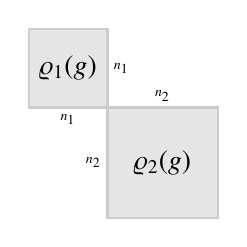
\begin{tikzpicture}[>=latex,thick]
\fill[color=white] (-1.2,-1.2) rectangle (1.2,1.2);
\fill[color=gray!20] (-1.2,1.2) rectangle (-0.2,0.2);
\draw[color=gray!40] (-1.2,1.2) rectangle (-0.2,0.2);
\node at (-0.7,0.25) [below] {\tiny $n_1$};
\node at (-0.25,0.7) [right] {\tiny $n_1$};
\node at (-0.7,0.7) {$\varrho_1(g)\mathstrut$};
\fill[color=gray!20] (-0.2,0.2) rectangle (1.2,-1.2);
\draw[color=gray!40] (-0.2,0.2) rectangle (1.2,-1.2);
\node at (0.5,-0.5) {$\varrho_2(g)\mathstrut$};
\node at (0.5,0.15) [above] {\tiny $n_2$};
\node at (-0.15,-0.5) [left] {\tiny $n_2$};
\end{tikzpicture}}\right).
\label{buch:gruppen:darstellungen:eqn:dirsummatrix}
\end{equation}
Diese Darstellung heisst die {\em direkte Summe} der Darstellungen
$\varrho_1$ und $\varrho_2$.
Für eine natürlich Zahl $k$ soll die
Schreibweise $k\cdot \varrho_1$ als die $k$-fache direkte Summe der
Darstellung $\varrho_1$ interpretiert werden.


%
% 63-vergleich.tex -- Vergleich von Darstellungen 
%
% (c) 2022 Prof Dr Andreas Müller, OST Ostschweizer Fachhochschule
%

%
% Vergleich von Darstellungen
%
\subsection{Vergleich von Darstellungen}
Die Einfachheit der regulären Darstellung hängt davon ab, dass man die
Basis sehr speziell wählen kann.
Eine beliebige Darstellung auf den ersten Blick sehr viel weniger gut
durchschaubar, weil eine beliebig gewählte Basis zu Matrizen führt,
die die Natur Gruppe verschleiern können.
Umgekehrt kann auch die reguläre Darstellung verbergen, dass dahinter
eigentlich einfachere Darstellungen stecken, die man besser erkennen
könnte, wenn man eine zweckmässigere Basis verwenden würde.
Das folgende Beispiel illustriert dies.

\begin{beispiel}
\label{buch:gruppen:darstellung:bsp:c3}
Wir betrachten die reguläre Darstellung der zyklischen Gruppe mit
drei Elementen $C_3=\{0,1,2\}$.
Die Gruppenelemente $1,2\in C_1$ werden in der regulären Darstellung
durch die Matrizen
\[
1\mapsto
P_1=
\begin{pmatrix}
0&0&1\\
1&0&0\\
0&1&0
\end{pmatrix}
\qquad\text{und}\qquad
2\mapsto
P_2
=
\begin{pmatrix}
0&1&0\\
0&0&1\\
1&0&0
\end{pmatrix}
=
P_1^2
\]
dargestellt.

Wir verwenden jetzt im Vektorraum $\mathbb{R}^3$, auf dem diese Matrizen
wirken, eine alternative Basis wie folgt:
\[
b_1
=
\frac{1}{\!\sqrt{3}}
\begin{pmatrix}1\\1\\1\end{pmatrix}
,
\qquad
b_2
=
\frac{1}{\!\sqrt{2}}
\begin{pmatrix*}[r]1 \\ -1 \\ 0\end{pmatrix*}
\qquad\text{und}\qquad
b_3
=
\frac{1}{\!\sqrt{6}}
\begin{pmatrix*}[r] 1\\1\\-2\end{pmatrix*}.
\]
Die Basis ist orthonormiert.
Die Wirkung der Matrix $P_1$ auf diesen Basisvektoren ist
\begin{align*}
P_1b_1
&=
b_1\\
P_1b_2
&=
\frac{1}{\!\sqrt{2}}
\begin{pmatrix*}[r]
0\\1\\-1
\end{pmatrix*}
=
(P_1b_2\cdot b_2) b_2
+
(P_1b_2\cdot b_3) b_3
=
-\frac{1}{2}
b_2
+
\frac{\!\sqrt{3}}{2}
b_3
\\
P_1b_3
&=
\frac{1}{\!\sqrt{6}}
\begin{pmatrix*}[r]
-2\\ 1\\1
\end{pmatrix*}
=
(P_1b_3\cdot b_2) b_2
+
(P_1b_3\cdot b_3) b_3
=
-\frac{\!\sqrt{3}}{2}
b_2
-
\frac{1}{2}
b_3
\end{align*}
Die Koeffizienten in der Darstellung der Bildvektoren in der
orthonormierten Basis $\{b_1,b_2,b_3\}$ auf der rechten Seite
können mit Hilfe des Skalarproduktes ermittel werden.
In der Basis $b_i$ bekommt die Matrix $P_1$ also die Matrix
\begin{equation}
\renewcommand{\arraystretch}{1.2}
\tilde{P}_1
=
\begin{pmatrix}
1&0&0\\
0&-\frac12 & \frac{\!\sqrt{3}}2\\
0&-\frac{\!\sqrt{3}}2&-\frac12
\end{pmatrix}
=
\begin{pmatrix}
1&0&0\\
0&\cos\bigl(-\frac{2\pi}{3}\bigr)& -\sin\bigl(-\frac{2\pi}{3}\bigr) \\
0&\sin\bigl(-\frac{2\pi}{3}\bigr)& \phantom{-}\cos\bigl(-\frac{2\pi}{3}\bigr)
\end{pmatrix}.
\label{buch:gruppen:darstellung:bsp:c3:blockform}
\end{equation}
In der neuen Basis zerfällt die Matrix in zwei Blöcke.
Der linke obere Block ist die eindimensionale triviale Darstellung.
der $2\times 2$-Block in der rechten unteren Ecke ist eine Drehmatrix mit
dem Drehwinkel $120^\circ$.

Geometrisch bedeutet die Blockform
\eqref{buch:gruppen:darstellung:bsp:c3:blockform}, dass man den
dreidimensionalen Raum in eine Gerade mit Richtung $b_1$ und
eine dazu senkrechte Ebene mit Basis $\{b_2,b_3\}$ aufteilen
kann.
Auf der geraden operiert die Gruppe $C_3$ trivial, der zweidimensionale
Unterraum ist eine zweidimensionale Darstellung der Gruppe $C_3$.
Es ist also gelungen, die reguläre Darstellung von $C_3$ zu zerlegen
in zwei einfachere Darstellungen.

Die reguläre Darstellung ist die direkte Summe der eindimensionalen
trivialen Darstellung und der zweidimensionalen Darstellung durch
Drehmatrizen.
\end{beispiel}.

Durch Wahl einer geeigneten Basis kann also eine Darstellung umgeformt
werden in eine andere.
Die Basistransformation mit der $n\times n$-Transformationsmatrix
$T:\mathbb{R}^n\to\mathbb{R}^n$ führt die 
Darstellung $\varrho\colon G\to\operatorname{GL}_n(\mathbb{R}$ über
in die Darstellung
\[
\tilde{\varrho}
\colon
G\to\operatorname{GL}_n(\mathbb{R})
:
g\mapsto T\varrho(g)T^{-1}.
\]
Tatsächlich ist $\tilde{\varrho}$ ein Homomorphismus, denn wir können
nachrechnen, dass
\begin{align*}
\tilde{\varrho}(e)
&=
T\varrho(e)T^{-1}
=
TIT^{-1}
=
I
\\
\tilde{\varrho}(gh)
&=
T\varrho(gh)T^{-1}
=
T\varrho(g)\varrho(h)T^{-1}
=
T\varrho(g)T^{-1}T\varrho(h)T^{-1}
=
\tilde{\varrho}(g)
\tilde{\varrho}(h).
\end{align*}

\begin{definition}
Zwei $n$-dimensionale Darstellungen $\varrho_1$ und $\varrho_2$
heissen isomorph, wenn es eine reguläre Matrix $T$ gibt derart, dass
$\varrho_1(g)=T\varrho_2(g)T^{-1}$ für alle $g\in G$.
\end{definition}


%
% 64-schur.tex -- Irreduzible Darstellungen und das Lemma von Schur
%
% (c) 2022 Prof Dr Andreas Müller, OST Ostschweizer Fachhochschule
%

%
% Irreduzible Darstellungen und das Lemma von Schur
%
\subsection{Irreduzible Darstellungen und das Lemma von Schur}
Das Beispiel~\ref{buch:gruppen:darstellung:bsp:c3} hat gezeigt, dass
es möglich ist, die reguläre Darstellung der Gruppe $C_3$ bis auf
Isomorphie in eine direkte Summe zweier einfacherer Darstellungen
zu zerlegen.
Ganz ähnlich wie uns die harmonische Analysis in die Lage versetzt,
Funktionen in Summen von einfacheren Funktionen zu zerlegen, sollte
es auch möglich sein, beliebige Darstellungen in eine Summe von
Bausteinen zu zerlegen.
Dazu muss aber zunächst der Idee der Zerlegbarkeit einer Darstellung
eine eindeutige Definition gegeben werden.

Die Zerlegung der Darstellung von $C_3$ im 
Beispiel~\ref{buch:gruppen:darstellung:bsp:c3} war möglich, weil
der Vektorraum $\mathbb{R}^3$ in zwei Summanden zerlegt werden 
konnte, die unter der Wirkung der Darstellung unverändert sind.
Die Ebene im Beispiel kann aber nicht mehr weiter in eindimensionale
Unterräume aufgespalten werden.

\begin{definition}
\label{buch:gruppen:darstellung:def:irreduzibel}
Eine Darstellung $\varrho\colon G\to \operatorname{GL}_n(\mathbb{R})$ 
heisst {\em irreduzibel}, wenn die einzigen Unterräume, die von allen
Matrizen $\varrho(g)$ in sich abgebildet werden, der Nullraum $\{0\}$
und der ganze Raum $\mathbb{R}^n$ sind.
\end{definition}

Nach dieser Definition ist die reguläre Darstellung von $C_3$ nicht
irreduzibel, da die beiden Unterräume
\[
\mathbb{R}b_1%\begin{pmatrix}1\\1\\1\end{pmatrix}
\qquad\text{und}\qquad
\{
xb_2 + yb_3
\mid
x,y\in\mathbb{R}
\}
\]
beide invariant sind.

\begin{satz}[Lemma von Schur]
\label{buch:gruppen:darstellung:satz:lemmavonschur}
Seien $G$ eine Gruppe sein $\varrho_V\colon G\to \operatorname{GL}(V)$
und $\varrho_W\colon G\to\operatorname{GL}(W)$ irreduzible Darstellungen
von $G$ in den Vektorräumen $V$ und $W$.
Sei ausserdem $f\colon V\to W$ eine lineare Abbildung, die mit den
Darstellungen vertauscht, also
\begin{equation}
f\circ \varrho_V(g) = \varrho_W(g)\circ f.
\label{buch:gruppen:darstellung:eqn:schur}
\end{equation}
Dann gilt
\begin{enumerate}
\item $f$ ist entweder die Nullabbildung oder ein Isomorphismus.
\item Falls $V=W$ ist, hat $f$ die Form $f(v)=\lambda v$ mit
$\lambda\in \mathbb{C}$.
\end{enumerate}
\end{satz}

\begin{proof}[Beweis]
Der Kern von $f$ ist der Unterraum
$\operatorname{ker}f = \{v\in V\mid f(v)=0\}$.
Für $v\in\operatorname{ker}f$ ist
$f(\varrho_V(g)v) = \varrho_W(g) f(v) = \varrho_W(g) 0=0$, also ist
$\varrho_V(g)\in\operatorname{ker}f$.
Der Kern von $f$ ist damit ein invarianter Unterraum der Darstellung
$\varrho_V$ von $G$.
Da $\varrho_V$ irreduzibel ist, ist $\operatorname{ker}f$ entweder
der ganze Raum, in diesem Fall ist $f=0$ oder der Kern ist $0$, in diesem
Fall ist $f$ injektiv.

Das Bild von $f$ ist der Unterraum
$\operatorname{im}f = \{f(v)\mid v\in V\}\subset W$.
Dann gilt wegen \eqref{buch:gruppen:darstellung:eqn:schur}
$\varrho_W(g)f(v) = f(\varrho_V(g)v)\in\operatorname{im}f$, das Bild von
$f$ ist damit auch ein invarianter Unterraum von $W$.
Da die Darstellung $\varrho_W$  irreduzibel ist, ist $\operatorname{im}f$
entweder der Nullraum, in diesem Fall ist $f=0$, oder das Bild ist der
ganze Raum $W$, in diesem Fall ist $f$ surjektiv.

Die beiden Aussagen zusammen ergeben, dass $f$ entweder die Nullabbildung
ist oder sowohl injektiv wie auch surjektiv ist.
Damit ist 1.~gezeigt.

Bleibt noch 2.~zu zeigen.
Sei $\lambda$ ein Eigenwert der Abbildung $f$ und $v$ ein Eigenvektor.
Dann ist $\lambda I$ eine
Abbildung $V\to V$, die mit der Darstellung vertauscht, denn
\[
\varrho_V(g)\lambda I =
\lambda \varrho_V(g) = \lambda I\varrho_V(g).
\]
Somit ist auch $f-\lambda I$ eine Abbildung $V\to V$, die mit $\varrho_V$
vertauscht.
Nach 1.~muss dies die Nullabbildung oder ein Isomorphismus sein.
Da aber der Eigenvektor $v$ auf $(f-\lambda I)v = \lambda v - \lambda v = 0$
abgebildet wird, kann $f-\lambda I$ nicht ein Isomorphismus sein, somit
ist $f-\lambda I=0$ und damit $f=\lambda I$.
\end{proof}

Die erste Aussage des Lemmas von Schur und sein Beweis zeigen, dass
irreduzible Darstellungen auch nicht teilweise aufeinander abgebildet
werden können.
Wenn eine Abbildung nicht die Nullabbildung ist, dann muss die
ganz Darstellung $V$ ohne Verlust auf die ganze Darstellung $W$
abgebildet werden.
Dies ist nur eine andere Formulierung für die Idee der Irreduzibilität.

Die zweite Aussage des Lemmas von Schur besagt im Wesentlichen, dass
es bis auf Faktor $\lambda$ nur eine Möglichkeit gibt, eine irreduzible
Darstellung mit sich selbst zu vergleichen.


%
% 65-charakter.tex -- Charakter einer Darstellung
%
% (c) 2022 Prof Dr Andreas Müller, OST Ostschweizer Fachhochschule
%

%
% Charakter einer Darstellung
%
\subsection{Charakter einer Darstellung}
Die reguläre Darstellung lässt die Gruppe auf Funktionen auf der
Gruppe operieren.
Der Begriff der irreduziblen Darstellung und das Lemma von Schur
lassen vermuten, dass nur sehr spezielle Funktionen für irreduzible
Darstellungen in Frage kommen.
Es ist daher eine Verbindung zwischen irreduziblen Darstellungen
und Funktionen auf der Gruppe herzustellen.
Diese Funktionen müssen unabhängig sein von der gewählten Basis.

\begin{definition}
\label{buch:gruppen:darstellungen:def:charakter}
Ist $\varrho_V\colon G\to\operatorname{GL}(V)$ eine Darstellung der
Gruppe $G$ im Vektorraum $V$, dann heisst die Funktion
\[
\chi_\varrho
\colon
G
\to
\mathbb{C}
:
g
\mapsto
\tr \varrho_V(g)
\]
der {\em Charakter} der Darstellung $\varrho$.
\end{definition}

Der Charakter einer Darstellung hängt nicht von der Wahl der Basis ab.
Zwei verschiedene Basen im Darstellungsraum $V$ führen auf verschiedene
Matrizen $\varrho_1(g),\varrho_2(g)\in\operatorname{GL}_n(\mathbb{C})$,
die aber durch eine Transformationsmatrix $T$ über die Formel
$\varrho_1(g)=T\varrho_2(g)T^{-1}$ miteinander verbunden sind.
Die Spur dieser Matrizen ist
\[
\tr \varrho_1(g)
=
\tr(T\varrho_2(g)T^{-1})
=
\tr(\varrho_2(g)T^{-1}T)
=
\tr \varrho_2(g),
\]
die Spuren sind also gleich.

Nicht jede Funktion kann ein Charakter sein, wie der folgende Satz
zeigt.

\begin{satz}
\label{buch:gruppen:darstellungen:satz:chareigenschaften}
Sei $\varrho$ eine $n$-dimensionale Darstellung von $G$ dann gilt
\begin{enumerate}
\item $\chi_\varrho(e) = n$
\item $\chi_\varrho(hgh^{-1}) = \chi_\varrho(g)$
\end{enumerate}
\end{satz}

\begin{proof}[Beweis]
Da $\varrho(e)=I_n$ die $n$-dimensionale Einheitsmatrix ist, ist
$\chi_\varrho(e) = \tr \varrho(e) = \tr I_n = n$, was 1.~beweist.
Aussage~3.~folgt aus
$\chi_\varrho(hgh^{-1})
=
\tr (\varrho(h)\varrho(g)\varrho(h)^{-1})
=
\tr \varrho(g)
=
\chi_\varrho(g)
$.
\end{proof}

Der Charakter einer Darstellung ist nur für eindimensionale Darstellungen
ein Homomorphismus, es ist also im Allgemeinen nicht möglich $\chi(g^{-1})$,
aus $\chi(g)$ zu berechnen.
Für endliche Gruppen gibt es aber einen Weg.

\begin{satz}
\label{buch:gruppen:darstellung:satz:charg-1}
Sei $\varrho$ eine $n$-dimensionale Darstellung einer endlichen Gruppe,
dann gilt
$\chi_\varrho(g^{-1}) = \overline{\chi_\varrho(g)}$.
\end{satz}

\begin{proof}[Beweis]
Wir verwenden eine Basis, in der die Matrix $\varrho(g)$ \JN hat.
Die \JN ist eine obere Dreiecksmatrix mit den Eigenwerten
$\lambda_i$ auf der Diagonalen.
Da spätestens die $n$-te Potenz von $g$ das neutrale Element ist und damit
die $n$-te Potenz der Matrix $\varrho(g)$ die Einheitsmatrix ist, müssen
alle Eigenwerte Betrag $1$ haben.
Die inverse Matrix $\varrho(g)^{-1}$ ist ebenfalls eine Dreiecksmatrix
mit den reziproken Eigenwerten $\lambda_i^{-1}$ auf der Diagonalen.
Da die $\lambda_i$ Betrag $1$ haben, ist $\lambda_i^{-1}=\overline{\lambda}_i$
und damit
\[
\chi_\varrho(g^{-1})
=
\tr \varrho(g^{-1})
=
\sum_{i=1}^n \lambda_i^{-1}
=
\sum_{i=1}^n \overline{\lambda}_i
=
\overline{\sum_{i=1}^n \lambda_i}
=
\overline{\tr \varrho(g)}
=
\overline{\chi_\varrho(g)}.
\]
\end{proof}

Der Beweis hängt davon ab, dass die Eigenwerte alle den Betrag $1$ haben,
eine Eigenschaft, die für eine endliche Gruppe dank der \JN leicht zu
erschliessen war.
Wir werden später sehen, dass man in vielen Fällen auch zeigen kann,
dass die Matrizen $\varrho(g)$ alle orthogonal oder unitär sind, was
ebenfalls zur Folge hat, dass die Eigenwerte Betrag $1$ haben.
Schliesslich kann auch die Einschränkung auf beschränkte Funktionen
ebenfalls Eigenwerte mit Betrag verschieden von $1$ ausschliessen.

%
%  Charaktere und Rechenoperationen mit Darstellungen
%
\subsubsection{Charaktere und Rechenoperationen mit Darstellungen}
In Abschnitt~\label{buch:gruppen:darstellungen:subsection:rechnen-mit-darstellungen}
wurden Rechenoperationen mit Darstellungen definiert.
Die direkte Summe $\varrho_1\oplus\varrho_2$ einer $n_1$-dimensionalen
Darstellung $\varrho_1$ und einer $n_2$-dimensionalen Darstellung
$\varrho_2$ ist eine $n_1+n_2$-dimensionale Darstellung.
Die Spur der Matrix~\eqref{buch:gruppen:darstellungen:eqn:dirsummatrix}
ist die Summe der Spuren der Teilmatrizen und daher
\[
\chi_{\varrho_1\oplus\varrho_2}
=
\chi_{\varrho_1}
+
\chi_{\varrho_2}.
\]

Wenn sich eine Darstellung in eine Summe von irreduziblen Darstellungen
zerlegen lässt, dann ist der Charakter der Darstellung die Summe der
Charaktere der irreduziblen Darstellungen.
Dies klingt wie eine Art harmonischer Analysis für Darstellungen: der
Charakter einer beliebigen Darstellung lässt sich zerlegen in eine
Linearkombination von Charakteren irreduzibler Darstellungen.

Um aus den Charakteren tatsächlich eine harmonische Analysis zu konstruieren,
müssen die Charaktere der irreduziblen Darstellungen bezüglich eines
geeigneten Skalarprodukts als Orthogonal erkannt werden.
Damit würde es möglich, beliebige Darstellungen einfach dadurch in
irreduzible Darstellungen zu zerlegen, dass man Skalarprodukte des
Charakters mit den Charakteren der irreduziblen Darstellungen bildet.


%
% 66-mittelung.tex -- Mittelung und mittelbare Gruppen
%
% (c) 2022 Prof Dr Andreas Müller, OST Ostschweizer Fachhochschule
%

%
% Mittelung und mittelbare Gruppen
%
\subsection{Mittelung und mittelbare Gruppen}
Harmonische Analysis vergleicht Funktionen mit Hilfe eines Skalarproduktes.
Für lokalkompakte topologische Gruppen, zu denen auch die endlichen Gruppen
zählen, haben wir das Haar-Mass, mit dem sich ein translationsinvariantes
Skalarprodukt definieren lässt.
Das Haar-Mass kann aber auch verwendet werden, um Mittelwerte zu bilden
und neue Darstellungen zu konstruieren.

Sei $f$ eine Funktion auf der Gruppe $G$ mit Werten in einem Vektorraum.
Die Gruppe operiert auf den Funktionen mit der Translation.
Eine Gruppe $G$ heisst {\em mittelbar}, wenn diese Operation gemittelt
\index{mittelbar}%
werden kann, wenn es also zu $f$ einen Mittelwert $Mf$ gibt, der 
translationsinvariant ist.
Falls $f$ bereits eine translationsinvariante Funktion ist, dann 
ist $Mf=f$.
Für eine endliche Gruppe kann man als {\em Mittelwert} einer Funktion
\index{Mittelwert}%
$f\colon G\to V$ das arithmetische Mittel
\[
Mf
=
\frac{1}{|G|}
\sum_{g\in G} T_gf
\]
verwenden.
Für eine lokal kompakte topologische Gruppe kann man die Mittelung
mit Hilfe des haarschen Masses als
\[
Mf
=
\int_G T_gf\,dg
\]
definieren, wobei dafür noch ein paar analytische Feinheiten der
Konvergenz geklärt werden müssten.
Um diesen Schwierigkeiten aus dem Weg zu gehen, werden wir im folgenden
die Aussagen nur für endliche Gruppen beweisen, auch wenn sie für
lokalkompakte topologische Gruppen mit kleinen Anpassungen ebenfalls
gültig sind.

Als erstes Beispiel für diese Idee zeigen wir, wie sich Darstellungen 
zerlegen lassen.
Wir verwenden dazu, dass Teilräume durch Projektionen beschrieben
werden können.

\begin{definition}[Projektion]
\label{buch:gruppen:darstellungen:def:projektion}
Eine {\em Projektion} in einem Vektorraum $V$ ist eine lineare Abbildung
$P\colon V\to V$ mit der Eigenschaft $P^2=P$.
\end{definition}

\begin{satz}
\label{buch:gruppen:darstellungen:satz:projektion}
Sei $\varrho\colon G\to\operatorname{GL}(V)$  eine endlichdimensionale
Darstellung der Gruppe $G$ und $W$ ein invarianter Unterraum von $V$,
also ein Unterraum, für den $\varrho(g)W\subset W$ für alle $g\in G$ gilt.
Dann gibt es einen invarianten Unterraum $W'$ mit $V=W\oplus W'$.
\end{satz}

\begin{proof}[Beweis]
Sei $W_0$ irgend ein komplementärer Unterraum mit $V=W\oplus W_0$, er muss
nicht invariant sein.
Zu dieser Zerlegung gibt es eine Projektionsabbildung $P\colon V\to V$ mit
$\operatorname{ker}P=W_0$ und $\operatorname{im}P=W$.
Auch die Abbildung $P$ muss nicht mit der Darstellung vertauschen.
Der Mittelwert 
\[
P'
=
\frac{1}{|G|}
\sum_{g\in G}
\varrho(g) P \varrho(g)^{-1}
\]
ist wieder eine lineare Abbildung.
Das Bild eines Vektors $v$ unter $P\varrho(g)^{-1}$ liegt in $W$ und wird
von $\varrho(g)$ wieder in $W$ abgebildet.
Da $W$ ein Unterraum von $V$ ist, ist somit $P'v\in W$.

Für Vektoren $w\in W$ hat $P$ die Eigenschaft $Pw=w$.
Daraus berechnet man
\[
P'w
=
\frac{1}{|G|}
\sum_{g\in G}
\varrho(g) P\varrho(g)^{-1}w
=
\frac{1}{|G|}
\sum_{g\in G}
\varrho(g) \varrho(g)^{-1}w
=
\frac{1}{|G|}
\sum_{g\in G}
w
=
w.
\]
Somit ist $P'$ eine Projektion $P^{\prime 2}=P'$ auf $W$.

Die Projektion $P'$ vertauscht aber zusätzlich mit der Darstellung, wie
wir jetzt nachrechnen wollen.
Es ist zu zeigen, dass $P'\varrho(h) = \varrho(h)P'$ für alle
Gruppenelemente $h\in G$.
Da die Multiplikation $g\mapsto hg$ eine Permutation der Gruppenelemente
ist, gilt auch
\begin{align*}
\varrho(h)P'\varrho(h)^{-1}
&=
\varrho(h)
\biggl(\frac{1}{|G|}\sum_{g\in G} \varrho(g)P\varrho(g)^{-1}\biggr)
\varrho(h)^{-1}
\\
&=
\frac{1}{|G|}
\sum_{g\in G} \varrho(hg)P\varrho(hg)^{-1}
\\
&=
\frac{1}{|G|}
\sum_{g\in G} \varrho(g)P\varrho(g)^{-1}
=
P'.
\end{align*}
Durch Multiplikation mit $\varrho(h)$ von rechts ergibt sich die Behauptung.

Somit ist $P'$ eine Projektion von $V$ auf $W$, die mit der Darstellung
vertauscht.
Der Kern von $P'$ ist $W'=\ker P'$ ist ebenfalls invariant, denn
\[
v\in\ker P'
\quad\Rightarrow\quad
P'
\varrho(g)v
=
\varrho(g)P'v
=
\varrho(g)0
=
0
\quad\rightarrow\quad
\varrho(g)v
\in \ker P'.
\]
Es folgt, dass $V=W\oplus W'$ eine komplementäre Zerlegung von $V$ in
invariante Unterräume ist.
\end{proof}

Das Argument kann analog auch für eine lokalkompakte topologische Gruppe
durchgeführt werden.
Die Eigenschaft der Mittelbarkeit zeigt also, dass zu einer Unterdarstellung
immer auch eine komplementäre Darstellung existiert.
Da die reguläre Darstellung immer die triviale Darstellung auf dem
eindimensionalen Unterraum der konstanten Funktionen als invarianten
Unterraum enthält, muss es einen komplementären invarianten Unterraum $W'$
geben derart, dass $\mathbb{C}[G]=\mathbb{C}\oplus W'$ ist.

\begin{satz}
\label{buch:gruppen:darstellungen:satz:abbmittel}
Seien $\varrho_i\colon G\to \operatorname{GL}(V_i)$ zwei irreduzible
Darstellungen von $G$ und $f\colon V_1\to V_2$ eine lineare Abbildung.
Setze
\[
f'
=
\frac{1}{|G|}
\sum_{g\in G} \varrho_2(g)^{-1}\circ f \circ \varrho_1(g).
\]
Dann ist $f'$ eine lineare Abbildung, die mit den Darstellungen vertauscht
und für die gilt:
\begin{enumerate}
\item Wenn die beiden Darstellungen nicht isomorph sind, dann ist $f'=0$.
\item Wenn $V_1=V_2$ und $\varrho_1=\varrho_2$, dann ist
$f'=\frac1n\tr(f)\cdot I_n$
mit $n=\dim V_1$.
\end{enumerate}
\end{satz}

\begin{proof}[Beweis]
Wir rechnen zunächst nach, dass $f'$ mit den Darstellungen vertauscht.
Dazu berechnen wir
\begin{align*}
\varrho_2(h)^{-1}f'\varrho_1(h)
&=
\varrho_2(h)^{-1}
\biggl(
\frac{1}{|G|}
\sum_{g\in G} \varrho_2(g)^{-1}f\varrho_1(g)
\biggr)
\varrho_1(h)
\\
&=
\frac{1}{|G|}
\sum_{g\in G}
\varrho_2(gh)^{-1} f \varrho_1(gh)
\\
&=
\frac{1}{|G|}
\sum_{g\in G}
\varrho_2(g)^{-1} f \varrho_1(g)
=
f',
\end{align*}
wobei im zweitletzten Schritt verwendet wurde, dass die Multiplikation
$g\mapsto gh$ eine Permutation in der Gruppe ist, die den Mittelwert
nicht ändert.
Durch Multiplikation von links mit $\varrho_2(h)$ folgt jetzt
$
f'\varrho_1(h) = \varrho_1(h)f'
$.

Auf die lineare Abbildung $f'$ können wir jetzt das Lemma von Schur
anwenden.
Es besagt, dass $f'$ entweder ein Isomorphismus ist oder eine
Nullabbildung, daraus folgt bereits 1.

Für die Spur von $f'$ gilt
\[
\tr f'
=
\frac{1}{|G|}
\sum_{g\in G} \tr\bigl(\varrho_1(g)^{-1} f\varrho_1(g)\bigr)
=
\frac{1}{|G|}
\sum_{g\in G} \tr f
=
f.
\]
Andererseits sagt das Lemma von Schur, dass $f'=\lambda I_n$ sein muss.
Die Spur davon ist $\tr f = \tr f' = \lambda \tr I_n = n\lambda$ oder
\[
\lambda = \frac1n \tr f
\qquad\Rightarrow\qquad
f' = \frac{1}{n} \tr(f)\cdot I_n
\]
Damit ist 2.~gezeigt.
\end{proof}


%
% 67-relationen.tex -- Algegraische Relationen für die Matrixelemente
%
% (c) 2022 Prof Dr Andreas Müller, OST Ostschweizer Fachhochschule
%

%
% Algebraische Relationen für die Matrixelemente
%
\subsection{Algebraische Relationen für die Matrixelemente}
Das Lemma von Schur hat noch mehr zu bieten.
Man kann damit nämlich sogar über die einzelnen Matrixelemente
einer Darstellung eine Aussage machen.
Ist $\varrho\colon G\to \operatorname{GL}_n(\mathbb{R})$ eine 
$n$-dimensionale Darstellung der Gruppe $G$, dann ist $\varrho(g)$
eine $n\times n$-Matrix bestehend aus den Matrixelementen
$(\varrho(g))_{ik}$ für $i,k=1,\dots,n$.

\begin{satz}
\label{buch:gruppen:darstellungen:satz:matrixnichtiso}
Wenn die Darstellungen $\varrho_i$ nicht isomorph sind, dann gilt
\begin{equation}
\frac{1}{|G|}
\sum_{g} \bigl(\varrho_1(g)^{-1}\bigr)_{i\!j} \bigl(\varrho_2(g)\bigr)_{kl}
=
0
\label{buch:gruppen:darstellungen:eqn:matrixnichtiso}
\end{equation}
für alle $i,j,k,l$.
\end{satz}

\begin{proof}[Beweis]
Wir schreiben die Resultate von
Satz~\ref{buch:gruppen:darstellungen:satz:abbmittel}
in Matrixform.
Die Abbildung $f$ hat die Matrixelemente $(f)_{i\!j}$.
Die Bedingung, dass $f'=0$ ist, bedeutet, dass alle
Matrixelemente $(f')_{il}=0$ sind.
Ausgeschrieben
\begin{align*}
(f')_{il}
&=
\frac{1}{|G|}
\sum_{g\in G}
\sum_{s,t}
\bigl(\varrho_2(g)^{-1}\bigr)_{is} (f)_{st} \bigl(\varrho_1(g)\bigr)_{tl}
\end{align*}
Nach 
Satz~\ref{buch:gruppen:darstellungen:satz:abbmittel}
ist dies immer $=0$, ganz unabhängig davon, was für Werte man für
die Matrix $f$ einsetzt.
Wählt man 
\begin{equation}
(f)_{st}
=
\begin{cases}
1&\qquad\text{$s=j$ und $t=k$}\\
0&\qquad\text{sonst},
\end{cases}
\qquad\text{oder}\qquad
(f)_{st}
=
\delta_{s\!j}\delta_{tk}
\label{buch:gruppen:darstellungen:eqn:fst}
\end{equation}
dann folgt
\[
0
=
\frac{1}{|G|}
\sum_{g\in G} 
\bigl(\varrho_2(g)^{-1}\bigr)_{is}
\delta_{s\!j}
\delta_{tk}
\bigl(\varrho_1(g)\bigr)_{kl}
=
\frac{1}{|G|}
\sum_{g\in G}
\bigl(\varrho_2(g)^{-1}\bigr)_{i\!j}
\bigl(\varrho_1(g)\bigr)_{kl}.
\]
Damit ist die Aussage bewiesen.
\end{proof}

\begin{satz}
\label{buch:gruppen:darstellungen:satz:matrixiso}
Sei $\varrho\colon G\to\operatorname{GL}(V)$ eine $n$-dimensionale
irreduzible Darstellung von $G$.
Dann gilt
\begin{equation}
\frac{1}{|G|}
\sum_{g\in G}
\bigl(\varrho(g^{-1})\bigr)_{i\!j} 
\bigl(\varrho(g))_{kl}
=
\frac1n
\delta_{il}\delta_{jk}
\label{buch:gruppen:darstellungen:eqn:matrixiso}
\end{equation}
\end{satz}

\begin{proof}[Beweis]
Mit der gleichen Notation wie im Beweis von
Satz~\ref{buch:gruppen:darstellungen:satz:matrixnichtiso}
schreiben wir das Resultat 2.~von
Satz~\ref{buch:gruppen:darstellungen:satz:abbmittel}
in Matrixform.
Es ist $f'=\frac1n \tr f$ und somit
\begin{equation}
(f')_{il}
=
\frac1n\tr(f)\delta_{il}
=
\frac{1}{|G|}
\sum_{g\in G}
\sum_{s,t}
\bigl(\varrho(g^{-1})\bigr)_{is}
f_{st}
\bigl(\varrho(g)\bigr)_{tl}.
\label{buch:gruppen:darstellungen:eqn:ff}
\end{equation}
Auch hier kann wieder $f$ beliebig gewählt werden.
Mit der Wahl
\eqref{buch:gruppen:darstellungen:eqn:fst}
$\tr f=\delta_{jk}$
wird

\eqref{buch:gruppen:darstellungen:eqn:ff} zu
\[
\frac1n \delta_{jk} \delta_{il}
=
\frac{1}{|G|}
\sum_{g\in G}
\sum_{s,t}
\bigl(\varrho(g^{-1})\bigr)_{is}
\delta_{s\!j}
\delta_{tk}
\bigl(\varrho(g)\bigr)_{tl}
=
\frac{1}{|G|}
\sum_{g\in G}
\bigl(\varrho(g^{-1})\bigr)_{i\!j}
\bigl(\varrho(g)\bigr)_{kl},
\]
wie behauptet.
\end{proof}

Beide Sätze besagen, dass ein ähnliches Konstrukt wie das Skalarprodukt
angewendet auf zwei verschiedene Matrixelemente immer entweder $0$
ergibt oder den Wert $1/n$.
Das Konstrukt, von dem hier die Rede ist, ist die Bildung
\[
(u,v)
=
\frac{1}{|G|}
\sum_{g\in G}
u(g^{-1}) v(g).
\]
Dies ist jedoch nicht das Skalarprodukt von Funktionen auf der
Gruppe.
Dazu müsste $u(g^{-1})=\overline{u(g)}$ sein, was im Allgemeinen
nicht zutrifft.
Wenn wir aber später zeigen können, dass es im Vektorraum ein Skalarprodukt
gibt derart, dass die Matrizen der Darstellung unitär sind, dann ist
$\bigl(\varrho(g^{1})\bigr)_{ik} = \overline{\varrho(g)_{ki}}$ und
$(u,v)$ stimmt mit dem Skalarprodukt der Matrixelemente überein.



%
% 68-orthochar.tex -- Orthogonalität der Charktere
%
% (c) 2022 Prof Dr Andreas Müller, OST Ostschweizer Fachhochschule
%

%
% Orthogonalität der Charaktere
%
\subsection{Orthogonalität der Charaktere}
Am Ende des vorangegangenen Abschnitts haben wir angedeutet, dass
die algebraischen Relationen zwischen den Matrixelementen einer
Darstellung fast wie Orthogonalitätsrelationen aussehen, dass die
Summe aber nicht das Skalarprodukt von Funktionen auf der Gruppe ist.
Charaktere von irreduziblen Darstellungen sind aber speziell und damit
ist es möglich, für Charaktere die folgenden Orthogonalitätsrelationen
zu beweisen.
Wir schreiben
\[
\langle \chi_1,\chi_2\rangle
=
\frac{1}{|G|} \sum_{g\in G} \overline{\chi_1(g)}\chi_2(g)
\]
für zwei Charaktere $\chi_1$ und $\chi_2$.

\begin{satz}
Ist $\chi$ der Charakter einer $n$-dimensionalen irreduziblen Darstellung,
dann ist $\langle \chi,\chi\rangle = 1$.
Sind $\chi_1$ und $\chi_2$ Charaktere von nichtisomorphen
irreduziblen $n_1$- bzw.~$n_2$-dimensionalen Darstellungen, dann 
ist $\langle \chi_1,\chi_2\rangle = 0$.
\end{satz}

\begin{proof}[Beweis]
Für den Charakter wissen wir aus
Satz~\ref{buch:gruppen:darstellung:satz:charg-1}, dass
$\chi(g^{-1}) = \overline{\chi(g)}$.
Dies bedeutet, dass wir in der Formeln
\eqref{buch:gruppen:darstellungen:eqn:matrixnichtiso}
und
\eqref{buch:gruppen:darstellungen:eqn:matrixiso}
die Inverse durch die komplexe Konjugation ersetzen können,
sofern wir die Formenl nur brauchen, um die Spur zu berechnen.

Das Skalarprodukt ist
\begin{align*}
\langle \chi_1,\chi_2\rangle
&=
\frac{1}{|G|}
\sum_{g\in G}
\overline{\chi_1(g)}
\chi_2(g)
=
\frac{1}{|G|}
\sum_{g\in G}
\chi_1(g^{-1})
\chi_2(g)
\\
&=
\frac{1}{|G|}
\sum_{g\in G}
\tr \varrho_1(g^{-1})
\cdot
\tr \varrho_2(g)
=
\frac{1}{|G|}
\sum_{g\in G}
\biggl(
\sum_{i}
\bigl(\varrho_1(g^{-1})\bigr)_{ii}
\biggl)
\cdot
\biggl(
\sum_{k}
\bigl(\varrho_2(g)\bigr)_{kk}
\biggl)
\\
&=
\sum_{i,k}
\frac{1}{|G|}
\sum_{g\in G}
\bigl(\varrho_1(g^{-1})\bigr)_{ii}
\bigl(\varrho_2(g)\bigr)_{kk}.
\intertext{Für nicht isomorphe Darstellungen verschwinden alle Summen
über die Gruppe und somit ist in diesem Fall $\langle \chi_1,\chi_2\rangle=0$.
Falls $\varrho_1=\varrho_2$ ist, also im Fall $\chi_1=\chi_2$ kann 
Formel~\ref{buch:gruppen:darstellungen:eqn:matrixiso}
mit $j=i$ und $l=k$ verwendet werden:}
&=
\sum_{i,k}
\frac1n\delta_{ik}\delta_{ik}
=
1.
\end{align*}
Damit ist die Orthonormierung der Charaktere bewiesen.
\end{proof}


%
% 69-orthouni.tex -- Orthogonale und unitäre Darstellungen
%
% (c) 2022 Prof Dr Andreas Müller, OST Ostschweizer Fachhochschule
%

%
% Orthogonale und unitäre Darstellungen
%
\subsection{Orthogonale und unitäre Darstellungen
\label{buch:gruppen:darstellung:subsection:orthouni}}
Im Beweis der Orthogonalität der Charktere war ein wesentlicher
Schritt die Erkenntnis, dass $\chi(g^{-1})=\overline{\chi(g)}$.
So eine Aussage fehlt uns bis jetzt und verunmöglicht damit, aus
den Sätzen
nicht nur Orthogonalitätsaussagen über die Spur, sondern über 
beliebige Paare von Matrixelementen zu gewinnen.
Eine solche Aussage ist auch nicht zu erwarten, denn die Gruppe
$G=\mathbb{R}$ hat die Darstellungen
\begin{equation}
\renewcommand{\arraycolsep}{3pt}
\begin{array}{rclclclcll}
\varrho_k
&\colon&
\mathbb{R} &\to& \operatorname{GL}_2(\mathbb{R})
&:&
t &\mapsto& \begin{pmatrix} \cos kt&-\sin kt\\\sin kt&\cos kt\end{pmatrix}
&\qquad k\in\mathbb{R}
\\
\psi
&\colon&
\mathbb{R} &\to& \operatorname{GL}_2(\mathbb{R})
&:&
t &\mapsto& \begin{pmatrix} t&0\\0&t^{-1}\end{pmatrix}.
&
\end{array}
\end{equation}
Die Matrizen $\varrho_k$ sind als Drehmatrizen alle orthogonal, die
Matrixelemente sind beschränkt und aus der klassischen Fourier-Theorie
sind Orthogonalitätsrelationen dafür bekannt.
Die Matrixelemente der Darstellung $\psi$ dagegen sind unbeschränkt und
man kann sich keine sinnvollen Orthogonalitätsrelationen vorstellen.

Die Orthogonalitätsrelationen der Matrixelemente von $\varrho_k$ 
im obigen Beispiel scheinen damit zusammenzuhängen, dass die Matrizen
$\varrho_k$ orthogonal sind.

\begin{definition}
Eine Darstellgung $\varrho\colon G\to\operatorname{GL}(V)$ einer
Gruppe in einem reellen Vektorraum $V$ mit einem Skalarprodukt
$\langle\;\,,\;\rangle$ heisst {\em orthogonal}, wenn
$\langle\varrho(g)u,\varrho(g)v\rangle=\langle u,v\rangle$
für alle $u,v\in V$.
Eine Darstellgung $\varrho\colon G\to\operatorname{GL}(V)$ einer
Gruppe in einem komplexen Vektorraum $V$ mit einem komplexen
Skalarprodukt $\langle\;\,,\;\rangle$ heisst {\em unitär}, wenn
$\langle\varrho(g)u,\varrho(g)v\rangle=\langle u,v\rangle$
für alle $u,v\in V$.
\end{definition}

\begin{beispiel}
Die Menge der reellwertigen Funktionen $\mathbb{R}[G]$ auf einer endlichen
Gruppe ist ein Vektorraum mit dem reellen Skalarprodukt
\[
\langle u,v\rangle
=
\frac{1}{|G|}
\sum_{g\in G} u(g)v(g),
\]
auf der die Gruppe durch die Translation $\varrho(h)=T_h$ wirkt.
Da die Multiplikation $g\mapsto hg$ nur eine Permutation der Gruppenelement
ist, bleibt das Skalarprodukt unter der Translation erhalten.
Somit ist die reguläre Darstellung orthogonal.

Die Menge der komplexwertigen Funktionen $\mathbb{C}[G]$ mit dem
komplexen Skalarprodukt 
\[
\langle u,v\rangle
=
\frac{1}{|G|}
\sum_{g\in G} \overline{u(g)} v(g)
\]
ist eine unitäre Darstellung von $G$ unter der Translation.
\end{beispiel}

\begin{satz}
Sei $\varrho\colon G\to\operatorname{GL}(V)$ eine reelle Darstellung
der endlichen Gruppe $G$ im $n$-dimensionalen Vektorraum $V$, dann gibt
es ein reelles Skalarprodukt $\langle \;\,,\;\rangle$ so, dass
$\varrho$ eine orthogonale Darstellung ist.
\end{satz}

\begin{proof}[Beweis]
Sei $(\;,\;)$ ein beliebiges reelles Skalarprodukt auf dem Vektorraum $V$,
es muss nicht invariant sein, es muss also nicht
\[
(\varrho(g)u,\varrho(g)v)
=
(u,v)
\]
gelten.
Das gemittelte Skalarprodukt
\[
\langle u,v\rangle
=
\frac{1}{|G|}
\sum_{g\in G}
(\varrho(g)u,\varrho(g)v)
\]
hat die Eigenschaft
\[
\langle \varrho(g)u,\varrho(g)v\rangle
=
\langle u,v\rangle,
\]
hat aber auch alle Eigenschaften eines reellen Skalarproduktes:
\begin{enumerate}
\item $\langle\;\,,\;\rangle$ ist symmetrisch:
\[
\langle u,v\rangle
=
\frac{1}{|G|} \sum_{g\in G} (\varrho(g)u,\varrho(g)v)
=
\frac{1}{|G|} \sum_{g\in G} (\varrho(g)v,\varrho(g)u)
=
\langle v,u\rangle
\]
für alle $u,v\in V$.
\item $\langle\;\,,\;\rangle$ ist bilinear:
\begin{align*}
\langle u_1+u_2,v\rangle
&=
\frac{1}{|G|} \sum_{g\in G} (u_1+u_2,v)
=
\frac{1}{|G|} \sum_{g\in G} (u_1,v)
+
\frac{1}{|G|} \sum_{g\in G} (_2,v)
=
\langle u_1,v\rangle + \langle u_2,v\rangle
\\
\langle \lambda u,v\rangle
&=
\frac{1}{|G|} \sum_{g\in G} (\lambda u,v)
=
\lambda
\frac{1}{|G|} \sum_{g\in G} (u,v)
=
\lambda \langle u,v\rangle.
\end{align*}
\item $\langle \;\,;\;\rangle$ ist positiv definit: für $v\in V\setminus\{0\}$:
\[
\langle v,v\rangle
=
\frac{1}{|G|} \sum_{g\in G}
\underbrace{(\varrho(g)v,\varrho(g)v)}_{\displaystyle > 0}
>
0.
\]
\end{enumerate}
Somit ist $\langle\;\,,\;\rangle$ ist ein invariantes Skalarprodukt und
die linearen Abbildung $\varrho(g)$ sind bezüglich dieses Skalarproduktes
orthogonal.
$\varrho(g)$ wird in einer bezüglich $\langle\;\,,\;\rangle$
orthonormierten Basis von $V$ durch eine orthogonale Matrix dargestellt.
\end{proof}

Da also zu einer Darstellung immer ein Skalarprodukt gewählt werden
kann, so dass die Darstellung orthogonal wird, kann man auch eine
orthonormierte Basis wählen und so erreichen, dass die Matrizen
$\varrho(g)$ in dieser Basis orthogonale Matrizen sind.
Eine orthogonale Matrix $O$ hat die Eigenschaft $O^{-1} = O^t$,
für die Matrixelemente $(\varrho(g))_{ik}$ gilt daher
\begin{equation}
\varrho(g^{-1})
=
\varrho(g)^{-1}
\qquad\Rightarrow\qquad
\varrho(g^{-1})_{ik}
=
\varrho(g)_{ki}.
\label{buch:gruppen:darstellungen:eqn:invorth}
\end{equation}
Ausserdem gelten für eine irreduzible Darstellung $\varrho$
weiterhin die Relationen
\eqref{buch:gruppen:darstellungen:eqn:matrixnichtiso}
und
\eqref{buch:gruppen:darstellungen:eqn:matrixiso}.
Setzt man \eqref{buch:gruppen:darstellungen:eqn:invorth} ein, erhält man
\begin{align*}
\frac{1}{n}
\delta_{il}\delta_{jk}
&=
\frac{1}{|G|}
\sum_{g\in G}
\bigl(\varrho(g^{-1})\bigr)_{ij}
\bigl(\varrho(g)\bigr)_{kl}
=
\frac{1}{|G|}
\sum_{g\in G}
\bigl(\varrho(g)\bigr)_{ji}
\bigl(\varrho(g)\bigr)_{kl}
=
\langle (\varrho)_{ji},\varrho_{kl}\rangle.
\end{align*}
Die Matrixelemente einer orthogonalen, irreduziblen Darstellung
sind also orthogonal.
Wir fassen das Resultat im folgenden Satz zusammen.

\begin{satz}
Ist $\varrho\colon G\to\operatorname{GL}(V)$ eine irreduzible,
$n$-dimensionale Darstellung im reellen Vektorraum $V$, dann gibt
es eine Basis von $V$ derart, dass $\varrho(g)$ durch orthogonale
Matrizen beschrieben werden.
Die Matrixelemente $\bigl(\varrho(g)\bigr)_{ik}$ sind orthogonale
Funktionen auf $G$.
\end{satz}

Mit der gleichen Methode kann ein entsprechendes Resultat für komplexe
Darstellungen der Gruppe $G$ gewonnen werden.

\begin{satz}
Sei $\varrho\colon G\to\operatorname{GL}(V)$ eine Darstellung der endlichen
Gruppe $G$ in einem komplexen endlichdimensionalen Vektorraum, dann gibt
es ein komplexes Skalarprodukt auf $V$ so, dass $\varrho$ eine unitäre
Darstellung ist.
\end{satz}

\begin{satz}
Sei $\varrho\colon G\to\operatorname{GL}(V)$ eine unitäre Darstellung
der endlichen Gruppe $G$ im komplexen Vektorraum $V$.
Die Matrixelemente $(\varrho(g))_{ik}$ in einer orthonormierten Basis
von $V$ sind orthogonale Funktionen auf $G$.
\end{satz}


%
% 6a-lie.tex -- Darstellungen von kompakten Lie-Gruppen
%
% (c) 2022 Prof Dr Andreas Müller, OST Ostschweizer Fachhochschule
%

%
% Darstellungen kompakter Lie-Gruppen
%
\subsection{Darstellungen kompakter Lie-Gruppen}
Die Resultate des letzten Abschnitts wurden jeweils nur für endliche Gruppen
beweisen.
In diesem Abschnitte sollen ein paar Hinweise zusammengetragen werden,
die illustrieren, wie die Resultate auch für die wichtige Klasse
der kompakten Lie-Gruppen, zu denen zum Beispiel die Drehgruppen
$\operatorname{SO}(n)$ und die unitären Gruppen $\operatorname{U}(n)$
gehören, erweitert werden können.
Dafür ist entscheidend, dass kompakte Lie-Gruppen ein rechts- und
linksinvariantes Haar-Mass haben.
Da die Gruppe kompakt ist, darf man sogar annehmen, dass das
Volumen
\[
\operatorname{vol}(G)
=
\int_G 1\, dg
\]
der Gruppe den Wert $1$ hat.
Für eine beliebige Funktion $f\colon G\to \mathbb{R}$ ist
\[
Mf
=
\int_G f(g)\,dg
\]
der Mittelwert der Funktion, die die für endliche Gruppen verwendete
normierte Summe $1/|G| \sum_{g\in G}f(g)$ als Mittelung ersetzen kann.

%
% Unitäre Darstellungen
%
\subsubsection{Unitäre Darstellungen}
Wie für eine endliche Gruppe kann man auch für eine endlichdimensionale
komplexe Darstellung $\varrho$ einer kompakten Lie-Gruppe auf einem
Vektorraum $V$ aus einem beliebigen Skalarprodukt $(\;,\;)$ auf $V$
ein invariantes Skalarprodukt mit der Mittelung
\begin{equation}
\langle u,v\rangle
=
\int_G (\varrho(g)u,\varrho(g)v)\,dg
\label{buch:gruppen:darstellungen:eqn:invskalarprodukt}
\end{equation}
konstruieren.
Die Konvergenz des Integrals ist für eine kompakte Lie-Gruppe immer 
gegeben.


%
% Eigenwerte
%
\subsubsection{Eigenwerte}
In Satz~\ref{buch:gruppen:darstellung:satz:charg-1} wurde gezeigt,
dass für den Charakter einer Darstellung einer endlichen Gruppe
$\chi(g^{-1})=\overline{\chi(g)}$ gilt.
Der Beweis hat gebraucht, dass die Eigenwerte komplexe Zahlen vom
Betrag $1$ sein mussten.

Das invariante Skalarprodukt
\eqref{buch:gruppen:darstellungen:eqn:invskalarprodukt}
zeigt, dass eine Darstellung einer kompakten Lie-Gruppe in einer
geeigneten Basis immer durch unitäre Matrizen möglich ist.
Die Wahl einer Basis hat aber keinen Einfluss auf die Eigenwerte.
Da unitäre Matrizen als Eigenwerte nur komplexe Zahlen vom Betrag $1$
haben können, folgt wie für endliche Gruppen, dass
$\chi(g^{-1})=\overline{\chi(g)}$ ist.

%
% Projektion
%
\subsubsection{Projektion}
In Satz~\ref{buch:gruppen:darstellungen:satz:projektion} wurde gezeigt,
dass zu einem invarianten Unterraum $W\subset V$ einer endlichdimensionalen
Darstellung $\varrho\colon G\to \operatorname{GL}(V)$ immer ein komplementärer
invarianter Unterraum $W'$ gefunden werden kann.
Der Beweis basierte auf der Idee, dass die Projektion $P\colon V\to W$,
die nicht unbedingt mit der Darstellung vertauschen muss, durch Mittelung
zu einer Projektion gemacht werden kann, die mit der Darstellung vertauscht.
Dies ist auch auf einer kompakten Lie-Gruppe möglich, man verwendet
\[
P'
=
\int_G \varrho(g)P\varrho(g)^{-1}\,dg,
\]
die Konvergenz des Integrals ist wieder durch die Kompaktheit der Gruppe
garantiert.
Damit folgt wieder, dass sich zu einem invarianten Unterraum $W\subset V$
eine direkte Zerlegung $V=W\oplus W'$ von Darstellungen finden lässt.

%
% Abbildungen zwischen Darstellungen
%
\subsubsection{Abbildungen zwischen Darstellungen}
In Satz~\ref{buch:gruppen:darstellungen:satz:abbmittel} wurde aus einer
linearen Abbildung $f\colon V_1\to V_2$ zwischen den Vekträumen zweier
Darstellungen $\varrho_i\colon G\to\operatorname{GL}(V_i)$ eine
gemittelte Abbildung 
\[
f
=
\int_G \varrho_w(g) \circ f \circ \varrho_1(g)\,dg
\]
konstruiert, die mit den Darstellungen vertauscht.
Die Schlussfolgerungen mit dem Lemma von Schur sind damit genau gleich
anwendbar zeigen, dass die Aussage von
Satz~\ref{buch:gruppen:darstellungen:satz:abbmittel} auch für kompakte
Lie-Gruppen gilt.

%
% Orthogonalitätseigenschaften
%
\subsubsection{Orthogonalitätseigenschaften}
Die Matrixform des Satzes~\ref{buch:gruppen:darstellungen:satz:abbmittel} 
hat auf Formeln der Sätze 
\ref{buch:gruppen:darstellungen:satz:matrixnichtiso}
und
\ref{buch:gruppen:darstellungen:satz:matrixiso}
ergeben, diese gelten jetzt auch für kompakte Lie-Gruppen.
Damit sind alle Voraussetzungen gegeben um zu schliessen, dass auch
die Orthogonalitätseigenschaften für die Charaktere von irreduziblen
Darstellungen und der Matrix-Elemente gelten.


%
% 6b-regulaer.tex -- Zerlegung der regulären Darstellung
%
% (c) 2022 Prof Dr Andreas Müller, OST Ostschweizer Fachhochschule
%

%
% Zerlegung der regulären Darstellung
%
\subsection{Zerlegung der regulären Darstellung
\label{buch:gruppen:darstellung:subsection:zerlegung}}
In der regulären Darstellung einer endlichen Gruppe operiert die
Gruppe durch Translation auf den Funktionen auf $G$.
Der Charakter einer irreduzible Darstellung sowie die Matrixelemente
sind ebenfalls Funktionen auf $G$.
Es stellt sich daher die Frage, ob die Charaktere oder die Matrixelemente
irreduzibler Darstellung dazu verwendet werden können, beliebige Funktionen
auf der Gruppe im Sinne der harmonischen Analysis mit dem Skalarprodukt
für Funktionen auf der Gruppe zu konstruieren.

\subsubsection{Der Charakter der regulären Darstellung}
Der Charakter der regulären Darstellung kann direkt berechnet werden,
wie der folgende Satz zeigt.

\begin{satz}
\label{buch:gruppen:darstellung:satz:regchar}
Sei $r_G$ der Charakter der reguläre Darstellung der Gruppe $G$ auf
$\mathbb{C}[G]$, dann gilt
\begin{equation}
r_G(g)
=
\begin{cases}
|G|&\qquad\text{falls $g=e$}\\
0  &\qquad\text{sonst.}
\end{cases}
\end{equation}
\end{satz}

\begin{proof}[Beweis]
Für die Berechnung des Charakters kann eine beliebige Basis verwendet
werden.
Für die früher verwendeten Basisvektoren $v_h$ mit $h\in G$ gilt
\[
T_gv_h = v_{gh}.
\]
Da $gh=h$ nur für $g=e$ gilt, sind die Diagonalelemente der Matrix $T_g$
für $g\ne e$ alle $=0$.
Für $g=e$ ist $T_g=T_e$ in der Basis $v_h$ die Einheitsmatrix $I_{|G|}$
und damit die Spur $\tr T_e = |G|$.
Damit ist die Aussage bewiesen.
\end{proof}

Seien jetzt $\varrho_1,\dots,\varrho_h$ die irreduziblen Darstellungen
von $G$ mit Dimension $n_1,\dots,n_h$ und Charakter $\chi_i$.
Die Charaktere sind orthonormierte Funktionen, daher kann die Zerlegung
der regulären Darstellung in irreduzible Summanden mit Hilfe des
Skalarproduktes durchgeführt werden.
Da wir den Charakter der regulären Darstellung in Satz
\ref{buch:gruppen:darstellung:satz:regchar}
vollständig berechnen konnten, lässt sich jetzt auch berechnen,
dass die irreduzible Darstellung $\varrho_i$ mit dem Charakter
der regulären Darstellung das Skalarprodukt
\[
\langle r_G,\chi_i\rangle
=
\frac{1}{|G|}
\sum_{g\in G} \overline{r_G(g)}\chi_i(g)
=
\frac{1}{|G|} r_G(e) \chi_i(e)
=
\frac{1}{|G|} |G| n_i
=
n_i
\]
hat.
Die Darstellung $\varrho_i$ kommt also $n_i$ mal in der regulären Darstellung
vor.

\begin{satz}
Die reguläre Darstellung enthält jede irreduzible $n$-dimensionale
Darstellung $n$ mal.
\end{satz}

Es folgt aber noch mehr. 
Der Charakter der regulären Darstellung kann als Linearkombination
\[
r_G(g)
=
\sum_{i=1}^h \langle \chi_i,r_G\rangle \chi_i(g)
=
\sum_{i=1}^h n_i \chi_i(g)
\]
geschrieben werden.
Aus dieser Formel folgt sofort der folgende Satz.

\begin{satz}
Die Dimensionen $n_i$ der irreduziblen Darstellungen von $n$ erfüllen
\[
\sum_{i=1}^n n_i^2 = |G|
\]
Die Werte $\chi_i(g)$ der Charaktere der irreduziblen Darstellungen erfüllen
für $g\ne e$ die Relation
\[
\sum_{i=1}^n n_i\chi_i(g) = 0.
\]
\end{satz}

%
% Zerlegung der regulären Darstellung
%
\subsubsection{Zerlegung der regulären Darstellung}
Die reguläre Darstellung enthält jede irreduzible Darstellung genau
so oft, wie die Dimension angibt.
In einer geeigneten Basis ist eine solche Darstellung unitär.
Die $n^2$ Matrixelemente sind orthogonal als Funktionen auf der Gruppe.
Die Matrixelemente bilden daher einen $n^2$-dimensionalen invarianten 
Unterraum der regulären Darstellung, dies sind genau die $n$
Kopien der zugehörigen irreduziblen Darstellung.

Die reguläre Darstellung lässt sich daher in eine Blockform bringen,
die für jede Darstellung $\varrho_i$ einen $n_i^2\times n_i^2$-Block
der Form
\[
T_g
=
\left(\raisebox{-2.95cm}{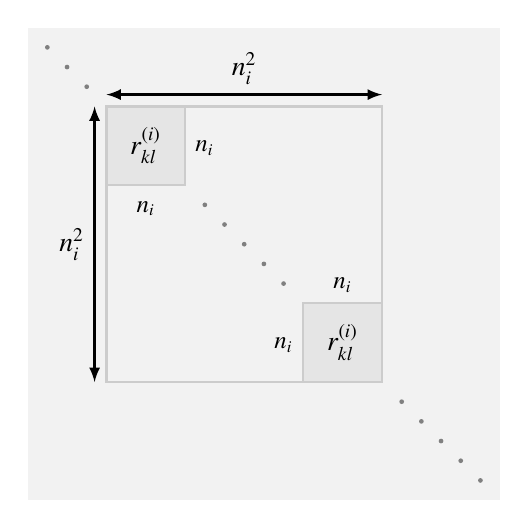
\begin{tikzpicture}[>=latex,thick]
\fill[color=gray!10] (-3,-3) rectangle (3,3);
\fill[color=gray!20] (-2,2) rectangle (-1,1);
\draw[color=gray!40] (-2,2) rectangle (-1,1);
\fill[color=gray!20] (0.5,-0.5) rectangle (1.5,-1.5);
\draw[color=gray!40] (0.5,-0.5) rectangle (1.5,-1.5);
\draw[color=gray!40] (-2,2) rectangle (1.5,-1.5);
\draw[color=gray!40] (-2,2) -- (-1.5,2);
\draw[color=gray!40] (0.5,-0.5) -- (1,-0.5);
\draw[color=gray!40] (0.5,-0.5) -- (0.5,-1);
\foreach \x in {2.75,2.5,2.25,0.75,0.5,0.25,0,-0.25,-1.75,-2,-2.25,-2.5,-2.75}{
	\fill[color=gray] (-\x,\x) circle[radius=0.03];
}
\node at (-1.5,1.5) {$r^{(i)}_{kl}$};
\node at (-1.5,1) [below] {\small $n_i\mathstrut$};
\node at (-1,1.5) [right] {\small $n_i\mathstrut$};
\node at (1,-1) {$r^{(i)}_{kl}$};
\node at (0.5,-1) [left] {\small $n_i\mathstrut$};
\node at (1,-0.5) [above] {\small $n_i\mathstrut$};
\draw[<->] (-2,2.15) -- (1.5,2.15);
\node at (-0.25,2.15) [above] {$n_i^2\mathstrut$};
\draw[<->] (-2.15,2) -- (-2.15,-1.5);
\node at (-2.15,0.25) [left] {$n_i^2\mathstrut$};
\end{tikzpicture}}
\right)
\]
enthält.
Jeder Block besteht aus $n_i$ identischen $n_i\times n_i$ Unterblöcken.
Die Matrixelemente $r^{(i)}_{kl}(g)$ dieser Unterblöcke bilden eine
orthonormierte Basis des Unterraumes der zu $\varrho_i$ isomorphen
Darstellungen in der regulären Darstellung.

\begin{beispiel}
Die zyklische Gruppe $C_n=\{0,\dots,n-1\}$ der Reste modulo $n$ hat $n$
Elemente.
Da sie abelsch ist, sind die irreduziblen Darstellungen eindimensional.
Da die Gruppe von $1$ erzeugt wird, ist die Darstellung $\varrho$ durch
das Element $\varrho(1)$ vollständig festgelegt.
Wegen $\varrho(n)=\varrho(0)=1$ muss $\varrho(n)=\varrho(1)^n =1$ sein,
d.~h.~$\varrho(1)=e^{2\pi ik/n}$ mit $k\in \{0,\dots,n-1\}$.
Die zugehörigen Funktionen auf $C_n$ sind  die Funktionen
$x\mapsto e^{2\pi ikx}$.
Aus der allgemeinen Theorie der Darstellungen folgt jetzt, dass diese
Funktionen bezüglich des Skalarproduktes
\[
\langle f,g\rangle
=
\frac{1}{n} \sum_{x=0}^{n-1} \overline{f(x)} g(x)
\]
orthonormiert sind.
Damit haben wir die Basisfunktionen der diskreten harmonischen
Analysis für die Gruppe $C_n$ aus der Darstellungstheorie wiedergewonnen.
\end{beispiel}

%
% Zerlegung der regulären Darstellung einer kompakten Lie-Gruppe
%
\subsubsection{Zerlegung der regulären Darstellung einer kompakten Lie-Gruppe}
Die Zerlegung der regulären Darstellung funktioniert auch für eine
Lie-Gruppe, was aber etwas aufwendiger zu beweisen ist.
Insbesondere ist es nicht sinnvoll, vom Charakter der regulären Darstellung
zu sprechen, da die reguläre Darstellung eine unendlichdimensionale 
Darstellung ist.
Es gilt aber weiterhin, dass endlichdimensionale irreduzible
Darstellungen genau dann isomorph sind, wenn ihr Skalarprodukt $1$ ist.
Auch die Matrixelemente einer $n$-dimensionalen irreduziblen Darstellungen
sind $n^2$ orthonormierte Funktionen, die eine Basis der $n$ in der
regulären Darstellung von $G$ vorkommenden Kopien der irreduziblen
Darstellung sind.

\begin{beispiel}
Die Gruppe $\mathbb{R}/2\pi\mathbb{Z}$ der Winkel ist abelsch.
Die Matrixelemente sind Funktionen, die unter der Translation invariant
sind, dies sind die Funktionen $x\mapsto e^{ikx}$ mit $k\in \mathbb{Z}$.
Als Skalarprodukt ist
\[
\langle f,g\rangle
=
\frac{1}{2\pi}
\int_0^{2\pi} \overline{f(x)}g(x)\,dx
\]
zu verwenden.
Die allgemeine Theorie zeigt dann, dass die Funktionen $e^{ikx}$ eine
orthonormierte Basis der integrierbaren Funktionen auf der $G$ ist.
Damit haben wir die Theorie der Fourier-Reihen aus der Darstellungstheorie
gewonnen.
\end{beispiel}








\section*{Übungsaufgabe}
\rhead{Übungsaufgabe}
\aufgabetoplevel{chapters/030-gruppen/uebungsaufgaben}
\begin{uebungsaufgaben}
\uebungsaufgabe{301}
\uebungsaufgabe{302}
%\uebungsaufgabe{102}
%\uebungsaufgabe{103}
%\uebungsaufgabe{104}
\end{uebungsaufgaben}

